\chapter{Experimental Setup and Results}
\label{ch:experimental-results}

%vTODO Add a section illustrating the implementation; giving some examples of how clustering algorithms are used to define a state-space and learn an MDP based on likelihood maximization and how this MDP is used to navigate the robot in an environment.

%\begin{itemize}
%	\item Introduction about application and high-level explanation of what we'll be looking into
%\end{itemize}

In \autoref{ch:methodology} a framework was proposed for finding an optimal \acrshort{acr:mdp} for planning problems that involve uncertainty given a dataset describing the dynamics of the system under consideration.
The framework aims to achieve this by posing the adjustment of the parameters of model learning algorithms as an optimization task in which the yielded performance is to be maximized.
The domain of mobile robot navigation, where the problem statement is to navigate a robot between locations as fast as possible, was identified as a potentially suitable application.
This chapter discusses the experiments that were conducted to evaluate the framework for this application and the results that were obtained accordingly.
First of all, \autoref{sec:setup} elaborates upon the setup for the experiments, discussing the relevant details on the implementation of the framework for this application and the software and other resources used.
Subsequently, \autoref{sec:scenarios} discusses the different configurations that are used to test the framework.
This, for instance, involves various combinations of learning algorithms and different settings of the weight factor $\beta$ on different environments.
In, \autoref{sec:results} the results obtained for these different configurations are presented, inspected and compared to one another, after which the most notable conclusions that can be drawn are discussed.

\section{Setup}
\label{sec:setup}

For our experiments we made an implementation of the framework in the form of a module that can be used to learn an optimal \acrshort{acr:mdp} for the navigation of a mobile robot.
This implementation allows the control of a mobile robot in simulations by an \acrshort{acr:mdp} and a corresponding policy.
The model values assessed from these simulations are used to find a globally maximizing parameter settings of the learning algorithm used.
In this section we will describe the implementation in detail and how it is used in our experiments to find performance-maximizing \acrshortpl{acr:mdp} for a mobile robot in an office environment.

\subsection{Software}
\label{sec:software}

In this section we discuss the software that is used in the implementation of our optimization module. 
An overview of the main packages used for this implementation is presented in \autoref{tab:software-packages}.
In the remainder of this section, we briefly explain for what part of the implementation each of these packages are used, and support the choices made where necessary.

\begin{table}[pt]
\caption{Software packages used for the implementation of the model learning framework for mobile robot navigation.}
\label{tab:software-packages}\centering
\begin{tabular}{|l|l|l|}
	\hline%
	\textbf{Package Name} & \textbf{Version} & \textbf{Purpose} \\
	\hline
	\texttt{bayesian-optimization} & 0.4.0 & Bayesian optimization \\
	\texttt{matplotlib} & 1.3.1 & Plotting and visualizing robot actions \\
	\texttt{pymdptoolbox} & 4.0\_b3 & \acrshort{acr:mdp} planning algorithms \\
	\texttt{ros-indigo-strands-desktop} & 0.0.14 & Simulation software and environments\\
	\texttt{scikit-learn} & 0.18.1 & Machine learning algorithms \\ \hline
\end{tabular}
\end{table}

\subsubsection{Python Libraries}

The module has been implemented in Python 2.7, due to its easily usable libraries for machine learning and plotting and other widely available packages, but also because of its convenient capability of interacting with the simulation software used.
An overview of the main software packages used for the implementation is shown in \autoref{tab:software-packages}.

\newpage

For \acrshort{acr:mdp} planning, the \texttt{pymdptoolbox} library \cite{cordwellpymdptoolbox}, is used, which implements various planning algorithms for discrete \acrshortpl{acr:mdp}. 
To solve for optimal policies in learned \acrshortpl{acr:mdp} we rely on this library and apply the \acrshort{acr:vi} algorithm with a discount factor of $\gamma = 0.95$.
%Given the matrices with the transition probabilities and rewards and algorithm-parameters like a discount factor $\gamma$, these planning algorithms can produce a policy vector and a corresponding value function.

For the machine learning algorithms used, we employ the \texttt{scikit-learn} library.
This library includes the implementations of $k$-Means clustering and the \acrshort{acr:em} algorithm for fitting \acrfullpl{acr:gmm}.

For \acrlong{acr:bo} the \texttt{bayesian-optimization} library \cite{nogueirabayesianoptimization} has been employed.
This library offers an implementation of the \acrshort{acr:bo} procedure based on a \acrshort{acr:gp} prior including the implementation of the most-used acquisition functions such as \acrshort{acr:mpi}, \acrshort{acr:mei} and \acrshort{acr:gp-ucb}.

%The further main Python packages used, have been listed in \autoref{tab:software-packages} and include \texttt{numpy} for the storage and manipulation of arrays and matrices used in the implementation and \texttt{matplotlib} for creating the various plots shown in this chapter.

\subsubsection{Simulator and Mobile Robot}

%vTODO Maybe remove these figures and rather show a figure of the simulator with the SCITOS robot?
% Make figure with two subfigures
%\begin{figure}[t]
%\centering
%\begin{minipage}{0.4\textwidth}
%	\centering
%	\vspace{21pt}
%	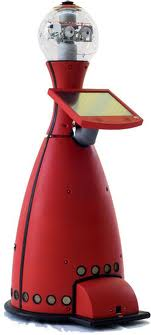
\includegraphics[width=0.3\linewidth]{scitosa5_1_model}
%	\vspace{4pt}
%	\captionof{figure}{The SCITOS-A5, mobile service robot by Metralabs GmbH \cite{Metralabs}}
%	\label{fig:scitosa5}
%\end{minipage}
%\qquad
%%%\begin{minipage}{0.4\textwidth}
%%%	\centering
%%%	\vspace{23pt}
%%%	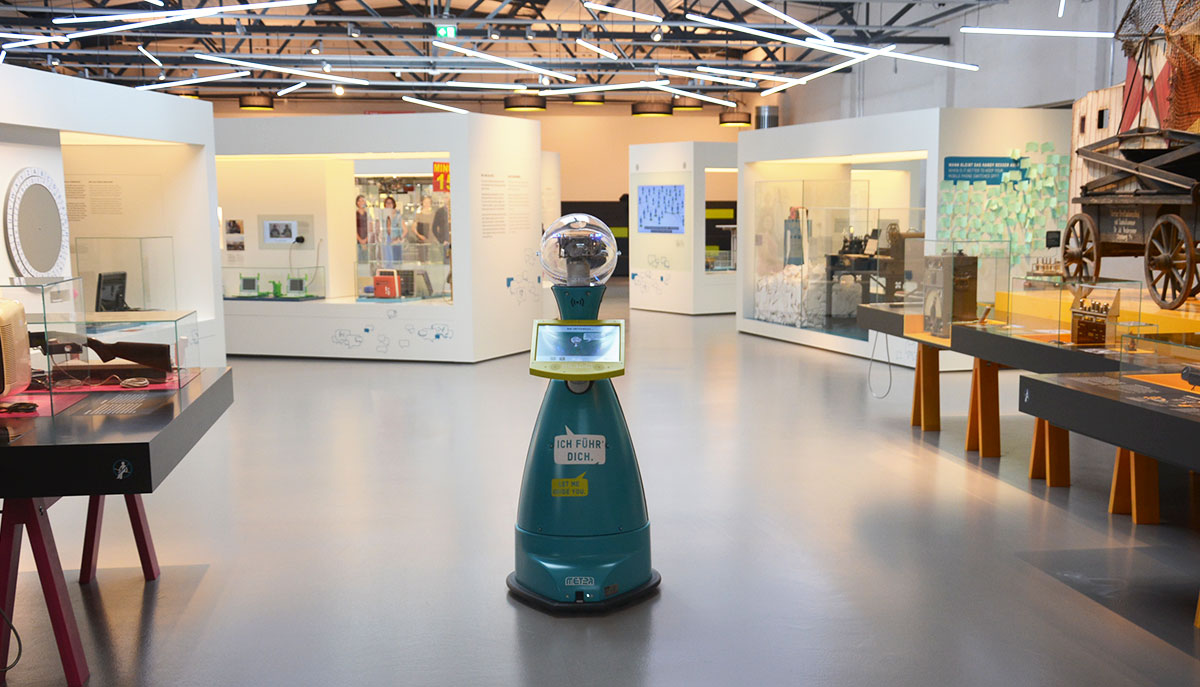
\includegraphics[width=1.1\linewidth]{scitosa5_2_TIM}
%%%	\vspace{-10pt}
%%%	\captionof{figure}{The SCITOS-A5 in one of its application environments. Shown here is robot \textit{TIM}, used for leading visitors of the German Technical Museum in Berlin through the exhibits \cite{Metralabs}.}
%%%	\label{fig:scitosa5_2}
%%%\end{minipage}
%\begin{minipage}{0.525\textwidth}
%	\centering
%	\vspace{10pt}
%	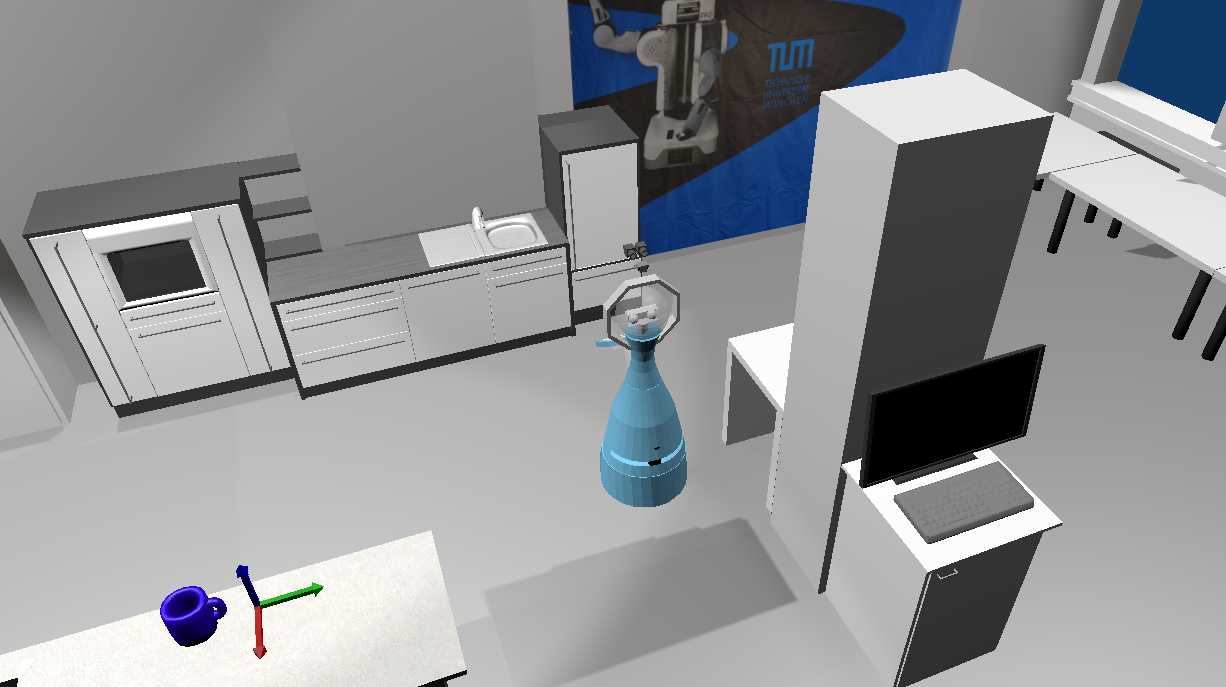
\includegraphics[width=1\linewidth]{simulator}
%	\vspace{-10pt}
%	\captionof{figure}{The SCITOS-A5 robot in a running MORSE simulation of the \texttt{tum\_kitchen} environment.}
%	\label{fig:simulator}
%\end{minipage}
%\quad
%\end{figure}

\begin{figure}[t]
	\centering
	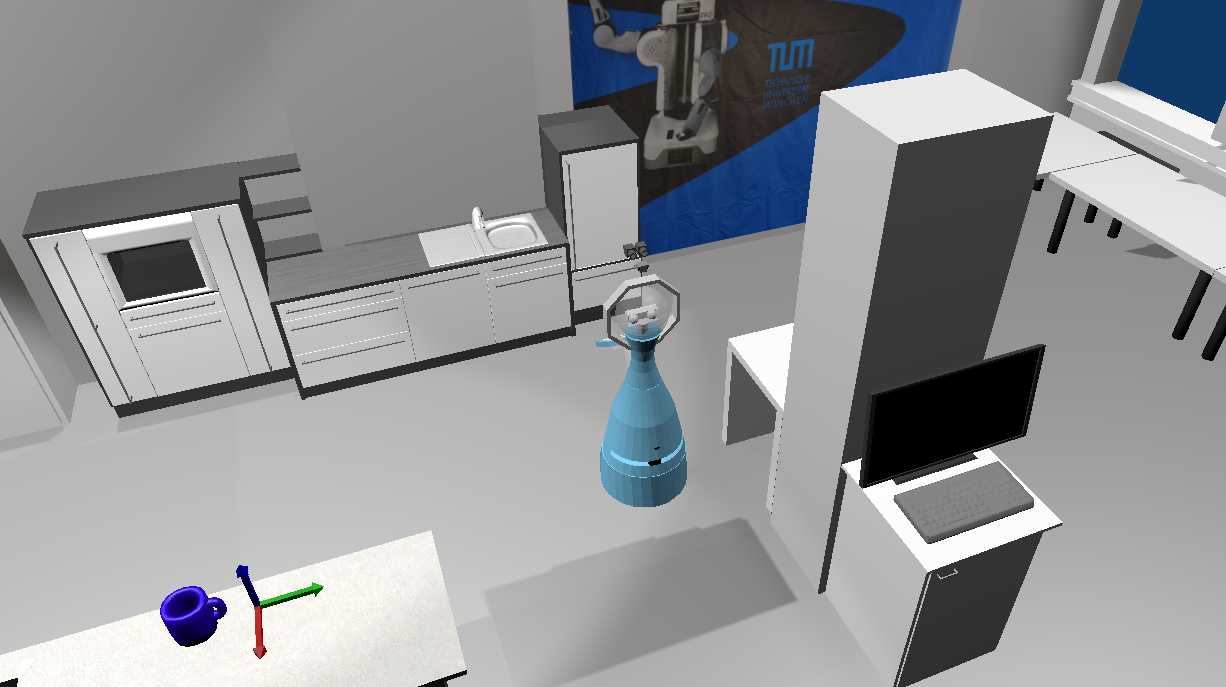
\includegraphics[width=0.65\linewidth]{simulator}
	\caption{The SCITOS-A5 mobile service robot in a running Morse simulation of the \texttt{tum\_kitchen} environment.}
	\label{fig:simulator}
\end{figure}

For performing simulations the \textit{MORSE} simulator \cite{morse_simpar_2012}, a generic simulator for academic robots, has been used in combination with the \textit{ROS} middleware to control the robot in an environment.
The simulations are performed with the Metralabs GmbH \textit{SCITOS-A5} \cite{Metralabs}, an industry-standard mobile service robot designed specifically for interacting with humans and guiding them to products or exhibits.
This robot is equipped with several sensors which can be used for navigation and \acrfull{acr:hri}, such as an omni-directional camera, 24 ultrasonic sensors, a collision sensor and a SICK laser range finder \cite{gross2008shopbot}.
As described in \autoref{sec:datasets} we are particularly interested in the odometric capabilities of the robot for the implementation that has been used in our experiments.
\autoref{fig:simulator} shows this robot in a MORSE simulation of one of the office environments used for our experiments.
The \texttt{strands-desktop} meta-package (developed as part of the \textit{STRANDS} project \cite{hawes2017strands}) was used to obtain all required simulation software mentioned above with ease, in which the environments used in the simulations of our experiments are contained as well.

%Software used for the implementation:
%\begin{itemize}
%	\item Programming Language: \textit{Python (2.7)} together with \texttt{scikit-learn}, \texttt{pymdptoolbox}, \texttt{bayesian-optimization} packages + explain what each of them are used for
%	\item Simulator: \textit{Morse}
%	\item Scitos-A5 robot, mobile service robot (plus \textit{short} discussion of what this robot has been used for in the real world)
%	\item Control movements of robot in simulator through \textit{ROS}
%\end{itemize}

\subsection{Dataset Acquisition}
\label{sec:datasets}

\begin{table}[pt]
	\caption{An excerpt of one of the execution traces datasets showing the format of the entries. Each entry stores the pose (\texttt{x}, \texttt{y} and \texttt{yaw}) of the robot based on odometry readings, and the action executed from this pose.}
	\label{tab:datasets-excerpt}\centering
	{\ttfamily
	\begin{tabular}{r|r|r|r}
		x & y & action\_id & yaw \\
		\hline
		2.243550300598145 & 3.1634166240692 & 1 & 0.7840424207077832 \\
		2.890618801116943 & 3.8128550052643 & 7 & -0.8159573629295891 \\
		3.541900634765625 & 3.1447956562042 & 6 & -1.6159579833378268 \\
		3.544688224792481 & 2.1472022533417 & 0 & -0.0326251734671011 \\
%		4.264401435852051 & 2.0662682056427 & 6 & -1.6326265827467716 \\
		... & ... & ... & ...
	\end{tabular}
	}
\end{table}

\begin{table}[pt]
	\caption{Details about the Morse simulation environments used and the size of the gathered datasets consisting of execution traces of the SCITOS-A5 robot.}
	\label{tab:datasets-environments}\centering
	\begin{tabular}{|l|r|r|}
		\hline
		\textbf{Environment Name} & \textbf{Approximate Area (\si{\metre\squared})} & \textbf{Number of Entries in Dataset} \\
		\hline
		\texttt{tum\_kitchen}& \num{100}              &   \num{4370}                                    \\
		\hline
		\texttt{uol\_bl}& \numrange[range-phrase = --]{800}{1000}               & \num{17245}           						\\ \hline          
	\end{tabular}
\end{table}

In order to be able to learn \acrshortpl{acr:mdp} from data and establish the optimization, we should obtain a dataset that  describes the environment the robot will operate in.
This dataset should describe possible robot poses and to what other poses the execution of the possible actions may lead to, in order to properly describe the dynamics of the system.

\newpage
For our implementation and the experiments that have been carried out, execution traces have been obtained by letting the robot follow a random action policy during which subsequent poses and actions are logged to a file.
This exploration is performed inside the simulator both for a relatively small environment (i.e., \texttt{tum\_kitchen}, based on a university kitchen of the Technical University of M\"unchen) and  large environment (i.e., \texttt{uol\_bl}, based on a floor in a faculty of the University of Lincoln) obtained from a repository of the \textit{STRANDS} project.

In the exploration a new entry is recorded in a file after each time-step of $t = \SI{1.0}{\second}$, which each contain the robot's pose based on odometric readings with its location as $x$ and $y$ position and its orientation described by the $yaw$.
Apart from that, each entry also stores the action that is executed next from the current pose.
As a result, the next entry tells us the robot's pose after the action in the previous entry has been executed.

In \autoref{tab:datasets-excerpt} an excerpt of one of the datasets is shown, which might give a clearer picture of the data that has been gathered and the format in which it has been stored.
The possible actions of the robot correspond to a discrete set of robot movements in $8$ different directions, being \textit{south}, \textit{south-east}, \textit{east}, \textit{north-east}, \textit{north}, \textit{north-west}, \textit{west} and \textit{south-west}.
For example, the first two entries describes the transformation of the robot's pose after trying to make a \textit{south-east} movement (n.b., positive difference in $x$ corresponds to moving south, while positive difference in $y$ corresponds to moving east).
\autoref{tab:datasets-environments} presents additional information about the environments and the size of the datasets gathered accordingly.

%Explain how the data-sets are obtained. 
%- For multiple environments - What is obtained. - How the data is obtained.

\subsection{Framework Implementation}
\label{sec:implementation}

To evaluate the framework proposed in \autoref{ch:methodology}, an implementation was made for the domain of mobile robot navigation.
This implementation optimizes for an \acrshort{acr:mdp} that maximizes the yielded performance of following plans derived from it. That is, it aims to find a model that ensures a mobile robot moves from one location in an environment to another as fast as possible.
In this section the relevant details of each part of the implementation are discussed.

\subsubsection{Learning Step}

For learning discrete-state \acrshortpl{acr:mdp} from the acquired execution traces, a likelihood maximization approach is applied based on a state space obtained from clustering algorithms.
That is, the state space is first obtained by applying a clustering algorithm (i.e., $k$-Means, \acrshort{acr:gmm}) with $\theta$ defining the number of components and the geometric positions of the execution traces as its training set.
Then, a transition probability distribution is fitted on the execution traces, such that an \acrshort{acr:mdp} may be obtained that comprehends the transitions that are possible when actions are performed from any of its states.

After having learned an \acrshort{acr:mdp}, the learning step next assesses the corresponding model value.
The model value is assessed based on how fast (i.e., expressed by the number of discrete time-steps) the agent would execute the tasks it is expected to perform when it is employed with the learned \acrshort{acr:mdp}.

For our domain we define each task as navigating from a start location to a goal location in the environment, each presented as a pair of coordinates, as fast as possible.
We translate these tasks into something that can be fed to the learned \acrshort{acr:mdp}, first of all, by setting the initial state of the \acrshort{acr:mdp} to the state predicted by the selected clustering algorithm for the start coordinates.
Similarly, a goal state is obtained, and accordingly a reward function for the \acrshort{acr:mdp} is defined as prescribed in \autoref{sec:learning-step}.
%by setting a one-time reward for this state.
%To avoid small state spaces (in which goal states do not map directly to true goals) yielding high value, a discrepancy factor is computed and used as described in \autoref{sec:learning-step}.

For each task, a value function and policy is computed for the \acrshort{acr:mdp} using the \acrshort{acr:vi} algorithm.
Based on the computed value functions and simulations following the corresponding policies, the value $V_\mathcal{M}$ of the learned \acrshort{acr:mdp} $\mathcal{M}$ is computed as in \autoref{eq:vm} of \autoref{sec:learning-step}.
In the simulations, for each task, the robot is first put at the start location defined by the task and then moves in the direction imposed by the computed policy at each discrete time-step.
It repeats this until the goal state has been reached.
At that point, however, the ``true'' goal might not have been reached by the robot.
This is a problem, because if we would quit the simulation as soon as the goal state has been reached, then \acrshortpl{acr:mdp} with state spaces that are too simple would yield high value.
To take this into account, as soon as the robot reaches the goal state, it checks if it is inside a designer-specified range of the goal location (i.e., the \textit{goal radius} in \autoref{tab:designer-settings}).
If not, the robot is moved into the direction of the goal location and the same check is performed.

To avoid the simulations running endlessly on a certain task, time-outs are defined at which the simulation is quit.
First of all, a (relatively short) \textit{goal time-out} is defined for reaching the goal from the goal state, which clearly cannot take too long.
Secondly, a \textit{stuck time-out} is defined, which starts when the robot remains at the same location after performing an action.
Finally, there is a \textit{global time-out}, that defines the maximum time the robot is allowed to spend on performing a task, taking into account any extra time caused by slipping.

The output of each learning step is the value of the learned model $V_\mathcal{M}$ and the time spent on model learning and planning.
The last being used when the \acrshort{acr:mei-ps} acquisition function is employed in the optimization.
Further, additional data is logged in each iteration, which is the total iteration time, simulation time, model learning time, total planning time and the parameter setting $\theta$ used.

%% IMPLEMENTATION LEARNING STEP
% Learning algorithm
	% Clustering algorithm
	% Maximum likelihood
% Objective: 
	% Learn MDP for given theta
	% Tasks (initial and goal locations)
	% Turned into reward function -> apply solver (VI) -> obtain value function and policy to use
	% Simulation:
		% Steps
		% Time-outs (1) stuck (2) goal state to reach goal (3) task
	% Output: Model value, time
% Logging

\begin{table}
	\caption{Settings for goal radius, parameter domain $\Theta$, time-outs and discount factor used for each of the environments in the experiments.}
	\label{tab:designer-settings}\centering
	\begin{tabular}{|l|r|r|r|r|r|r|}
		\hline
		\textbf{Environment} & \textbf{Goal Radius} & \textbf{Parameter} & \textbf{Goal T/O} & \textbf{Stuck T/O} & \textbf{Global T/O} & \textbf{Discount}  \\
		
		& \textbf{(\si\meter)} & \textbf{Domain $\Theta$} & (\si{\second}) & (\si{\second}) & (\si{\second}) & \textbf{Factor $\gamma$}\\
		\hline
		\texttt{tum\_kitchen} & \num{0.5} & $[2, 300]$ & \num{10} & \num{10} & \num{30} & \num{0.95} \\
		\hline
		\texttt{uol\_bl} & \num{1.0} & $[100, 1000]$ & \num{10} & \num{10} & \num{120} & \num{0.95}\\
		\hline
	\end{tabular}
\end{table}

\subsubsection{Optimization Step}

For the implementation of the framework for this domain we make use of the \acrshort{acr:bo} framework for optimization based on a \acrshort{acr:gp} with a Mat\'ern 3/2 kernel where the noise in the simulations is approximated by adding Gaussian white noise through a White kernel with estimated noise~level of $10^{-4}$.
As initially there is no knowledge about the model value given a parameter setting $\theta$, first, a number of random settings are selected for which yielded performance is assessed and stored in an evidence set.
In the following iterations new settings for $\theta$ are chosen with maximum utility in the selected acquisition function, which is repeated for a fixed number of iterations.

The first phase of the multi-phase framework described in \autoref{sec:multi-phase-framework} is executed as an individual optimization procedure, where the model values $V_\mathcal{M}$ are solely based on computed value functions and no simulations are performed.
The resulting posterior of this first phase is then used in the acquisition of the first few samples in the second phase with the aim of finding a global maximizer faster.

%% OPTIMIZATION STEP
% Initial points (random points)
% Stopping criterions


%Details on the implementation; how the framework/routine is implemented for this application. Discuss how the following aspects are taken care of in the implementation:
%\begin{itemize}
%	\item Environments
%	\item Exploration / Data Gathering
%	\item Optimization
%	\item Simulations of following policy
%\end{itemize}

\afterpage{
	\begin{figure}
		\centering
		%\captionsetup{font=small}
		\captionsetup[subfigure]{font=footnotesize}
		%\captionsetup[subfigure]{justification=centering}
		\begin{subfigure}{\textwidth}
			\centering
			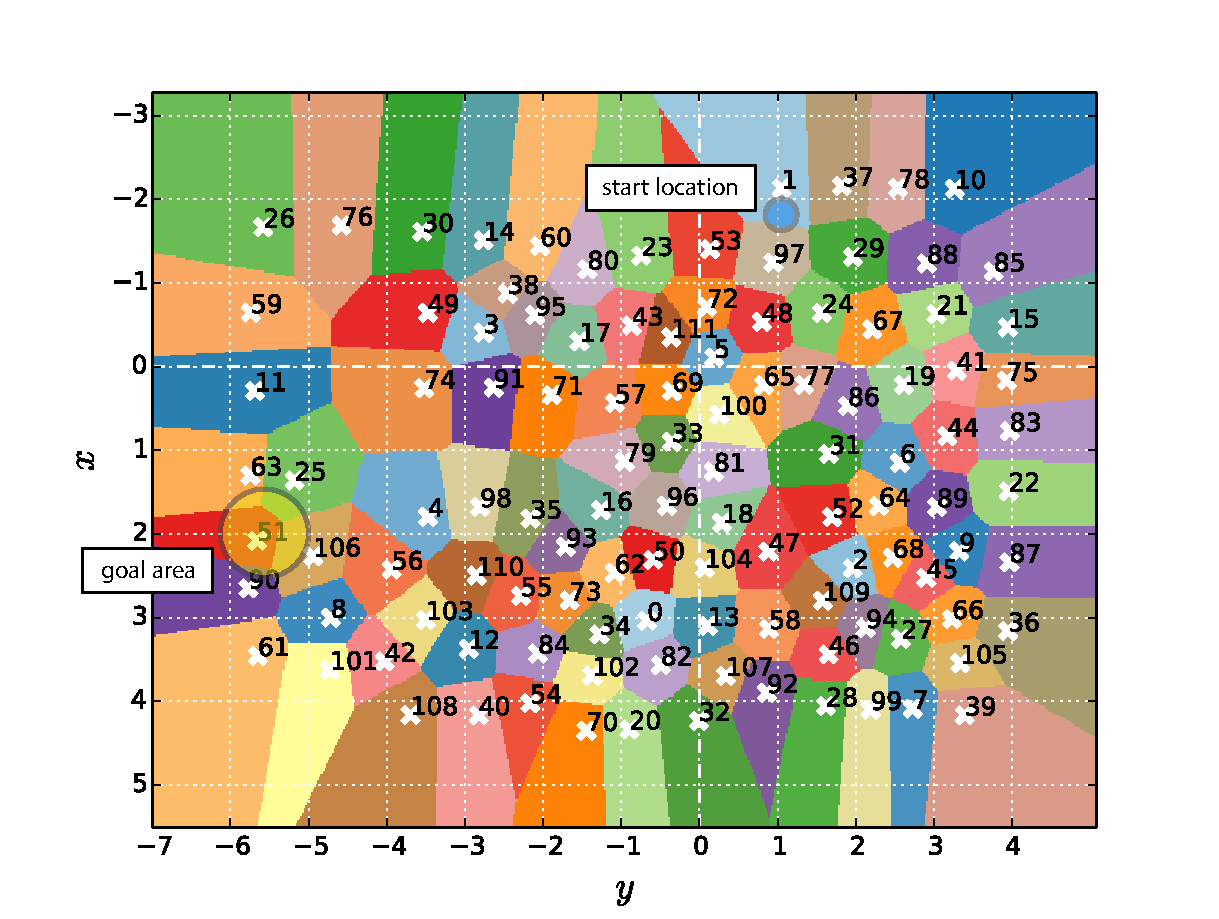
\includegraphics[width=\linewidth]{demo_clustering_v2}
			\caption{State space of an \acrshort{acr:mdp} with $112$ states for the \texttt{tum\_kitchen} environment learned by $k$-Means clustering. The plot depicts one of the tasks the mobile robot is expected to perform. The start location maps to a single state, labeled `$\mathsf{1}$'. The goal center maps to the state labeled `$\mathsf{51}$', while the goal area intersects with multiple states.}
			\label{fig:demo-clustering}
		\end{subfigure}
		
		\bigskip
		
		\begin{subfigure}{\textwidth}
			\centering
			%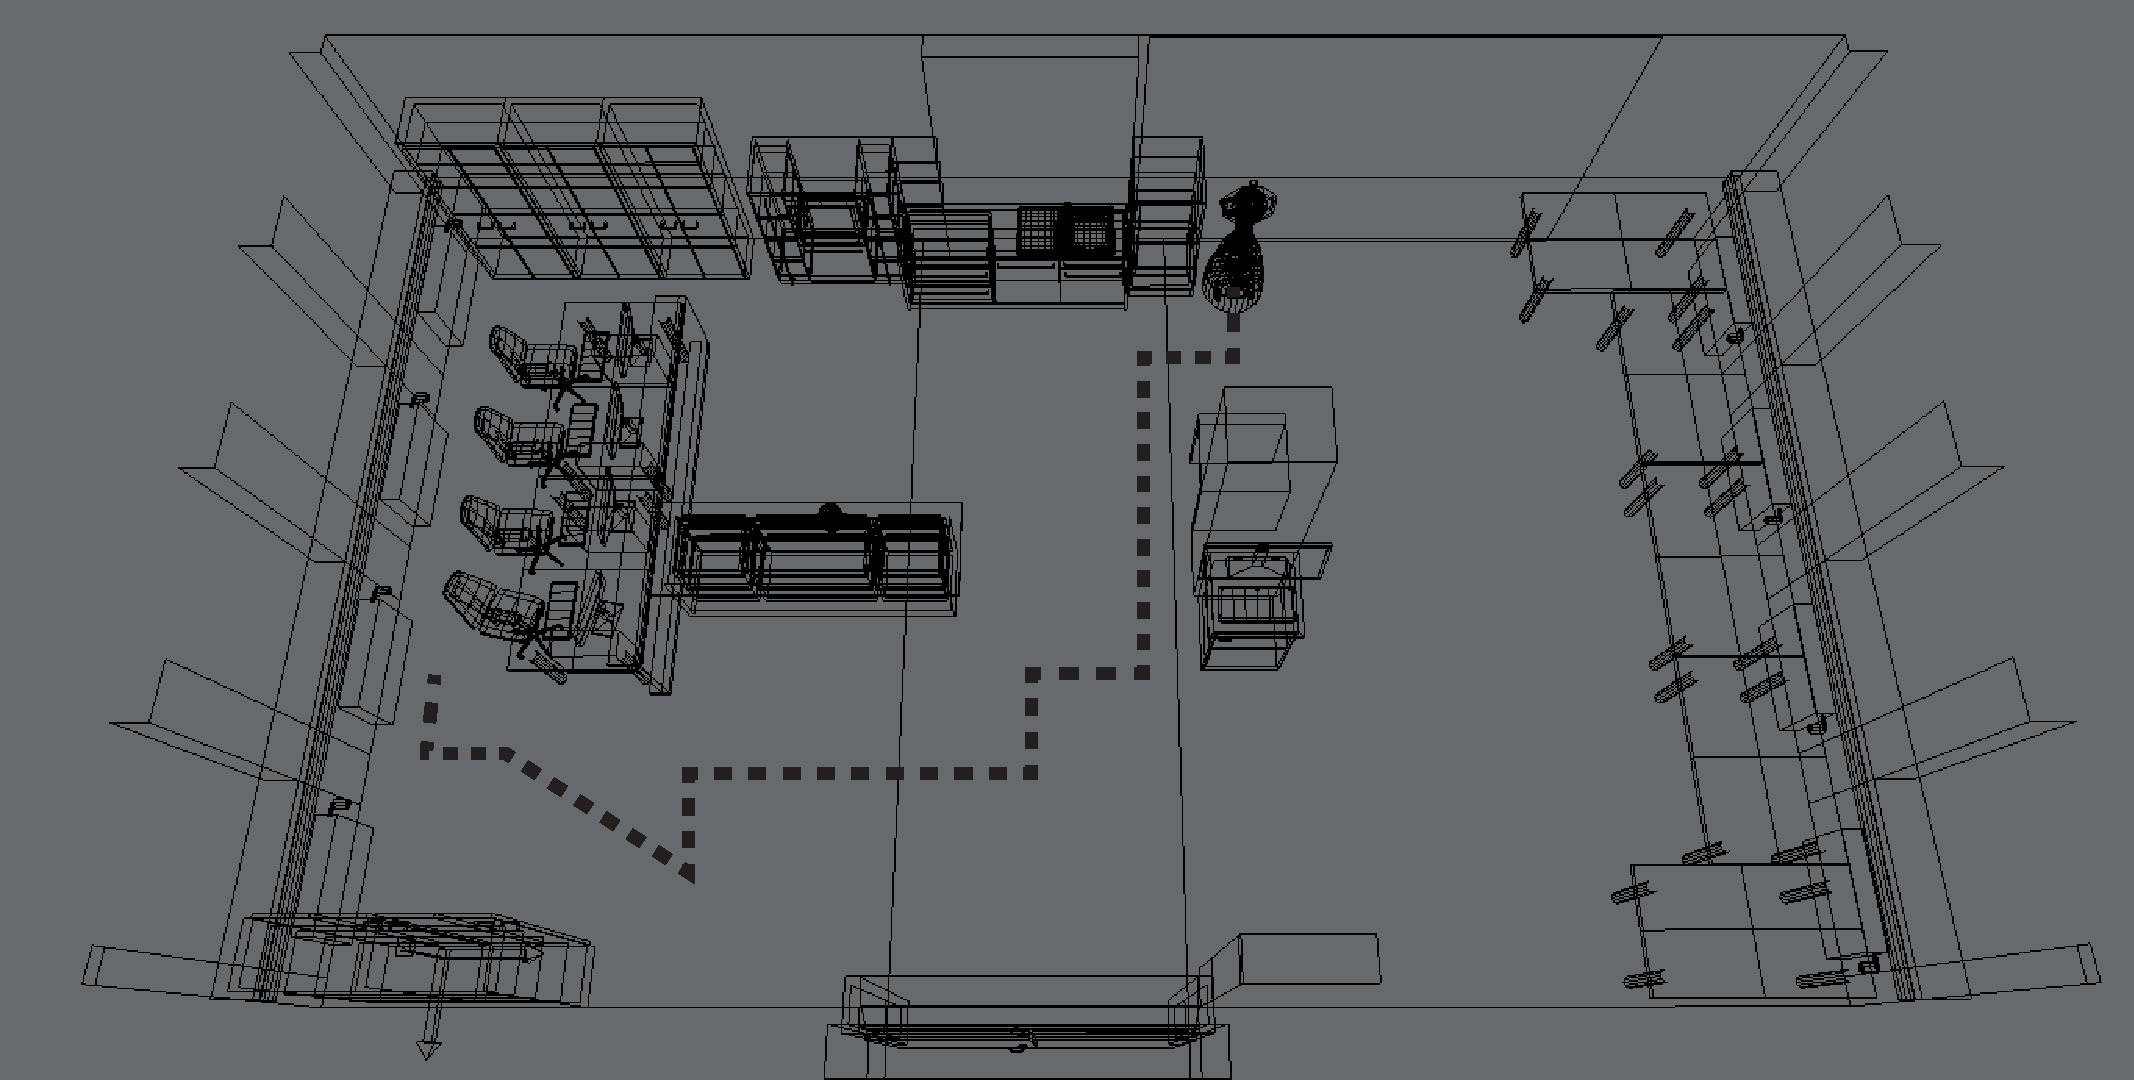
\includegraphics[width=\linewidth]{trajectory_v4}
			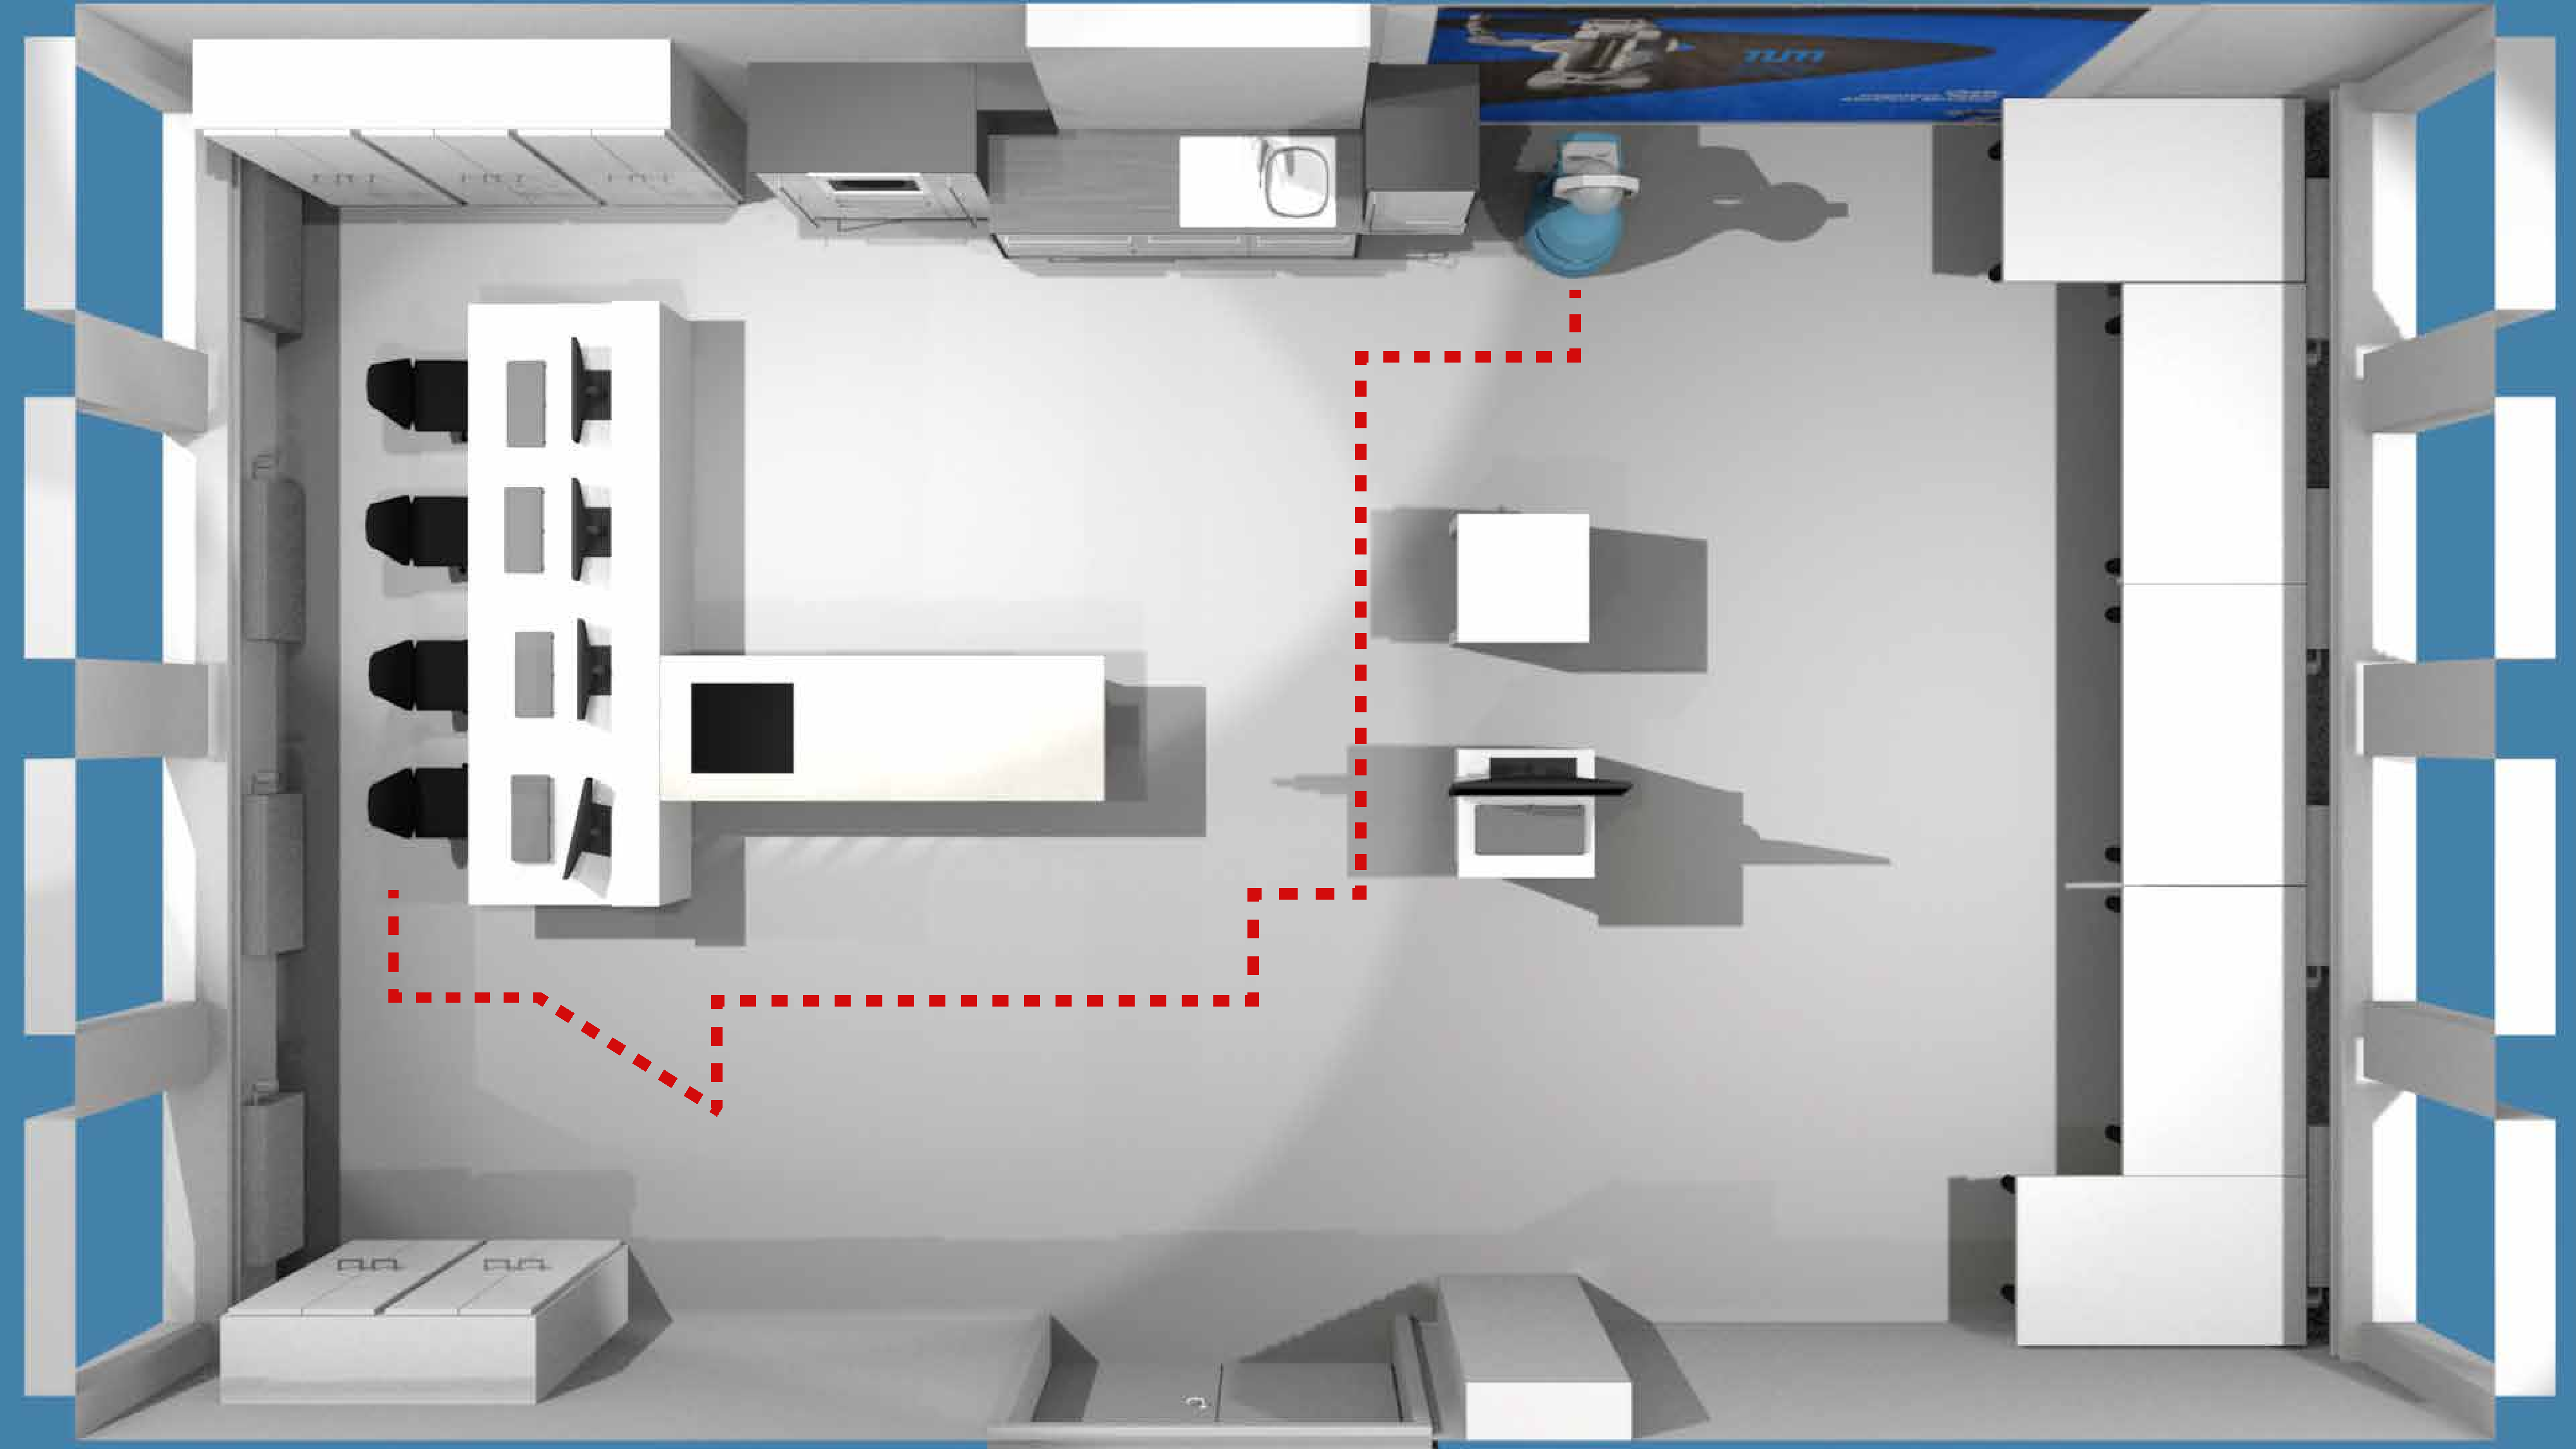
\includegraphics[width=\linewidth]{tum_kitchen_render_trajectory_v5_2}
			\caption{A MORSE simulation of the \texttt{tum\_kitchen} environment, showing the trajectory the SCITOS-A5 robot will follow to accomplish the task depicted in \autoref{fig:demo-clustering} according to the policy computed from the \acrshort{acr:mdp} using the \acrshort{acr:vi} algorithm.}
			\label{fig:demo-trajectory}
		\end{subfigure}
		\bigskip
		
		\caption{Demonstration of the implementation learning the state space of an \acrshort{acr:mdp} and using it for path planning for a task in the \texttt{tum\_kitchen} environment.}
		\label{fig:demonstration}
	\end{figure}
	\clearpage
}

\newpage

\subsection{Demonstration}
\label{sec:demonstration}

To provide the reader with a better insight as to how the implementation utilizes execution traces to learn \acrshortpl{acr:mdp} and use these for path planning, a demonstration is given of a single iteration of the framework, supported by the illustrations in \autoref{fig:demonstration}.
For this demonstration, let us assume that the optimization step provides us with a new parameter setting $\theta = 112$, specifying the number of states of the \acrshort{acr:mdp}, to evaluate.

First, given this parameter setting, a state space $\mathcal{S}$ is, in this case, learned by a $k$-Means clustering on the execution traces $E$, with the result shown in \autoref{fig:demo-clustering}.
Correspondingly, the transition function $\delta$ is fitted by maximum likelihood and a set of tasks $T$ are mapped to this state space.
To illustrate, let us take the task of moving from the position $(-1.9, 1.05)$ to $(2.0, -5.6)$, mapping to the states labeled with `$\mathsf{1}$' and `$\mathsf{51}$' respectively as shown in \autoref{fig:demo-clustering}.
Translating this into an initial state $s_0$ and reward function $R$, as described in \autoref{sec:learning-step}, results in an \acrshort{acr:mdp} $(\mathcal{S}, s_0, A, \delta, R)$ that can be solved using the \acrshort{acr:vi} algorithm to obtain a policy (and value function).
Then, to assess the performance in the simulator, this policy is employed, so that the robot will follow the trajectory as shown in \autoref{fig:demo-trajectory} (n.b., additionally, the robot might slip, so that it slightly deviates from this path).
Then, with $n$ being the recorded total number of time-steps, a performance measure for this task is obtained through \autoref{eq:vsim}.

%\begin{figure}[t!]
%	\centering
%	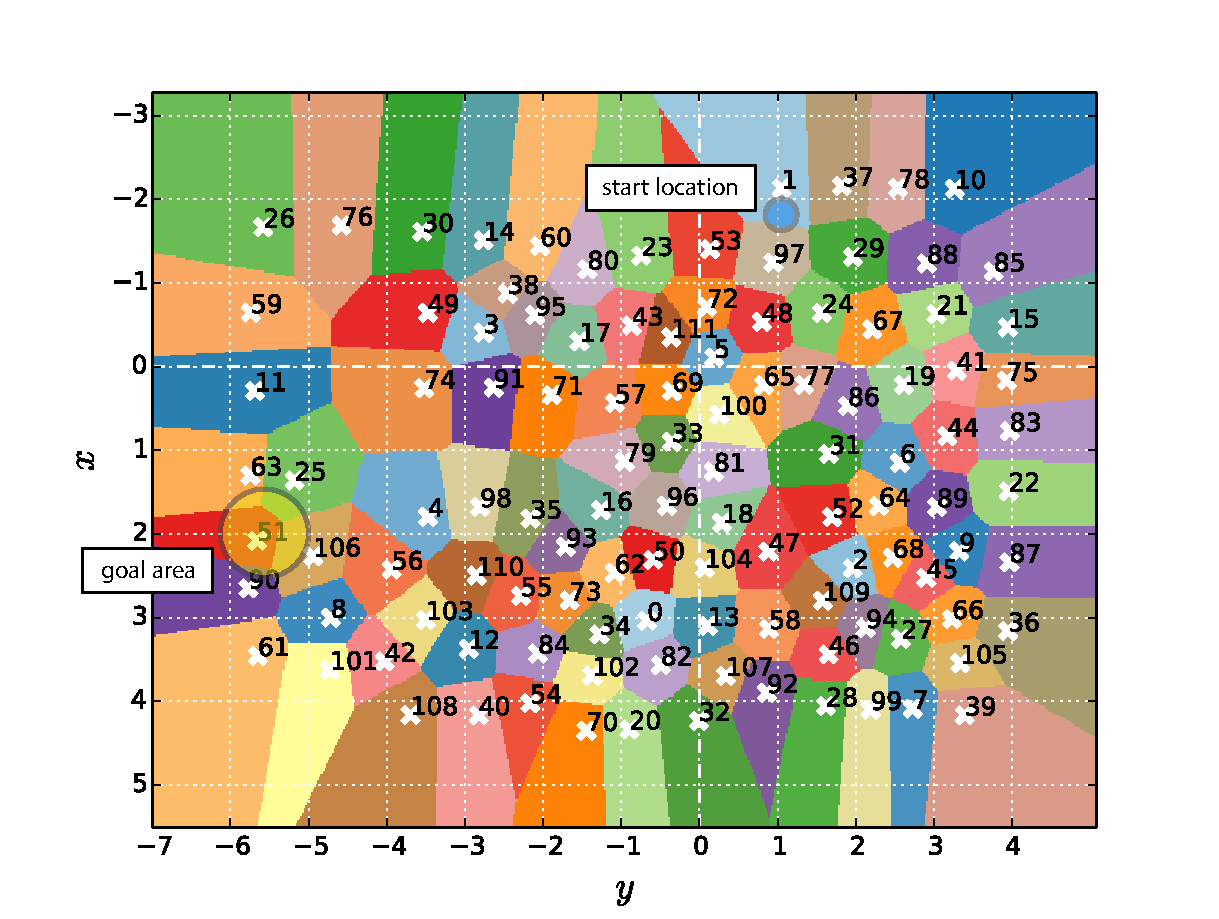
\includegraphics[width=0.9\textwidth]{demo_clustering_v2}
%	\caption{Clustering}
%	\label{fig:demo-clustering}
%\end{figure}
%
%\begin{figure}[t!]
%		\centering
%		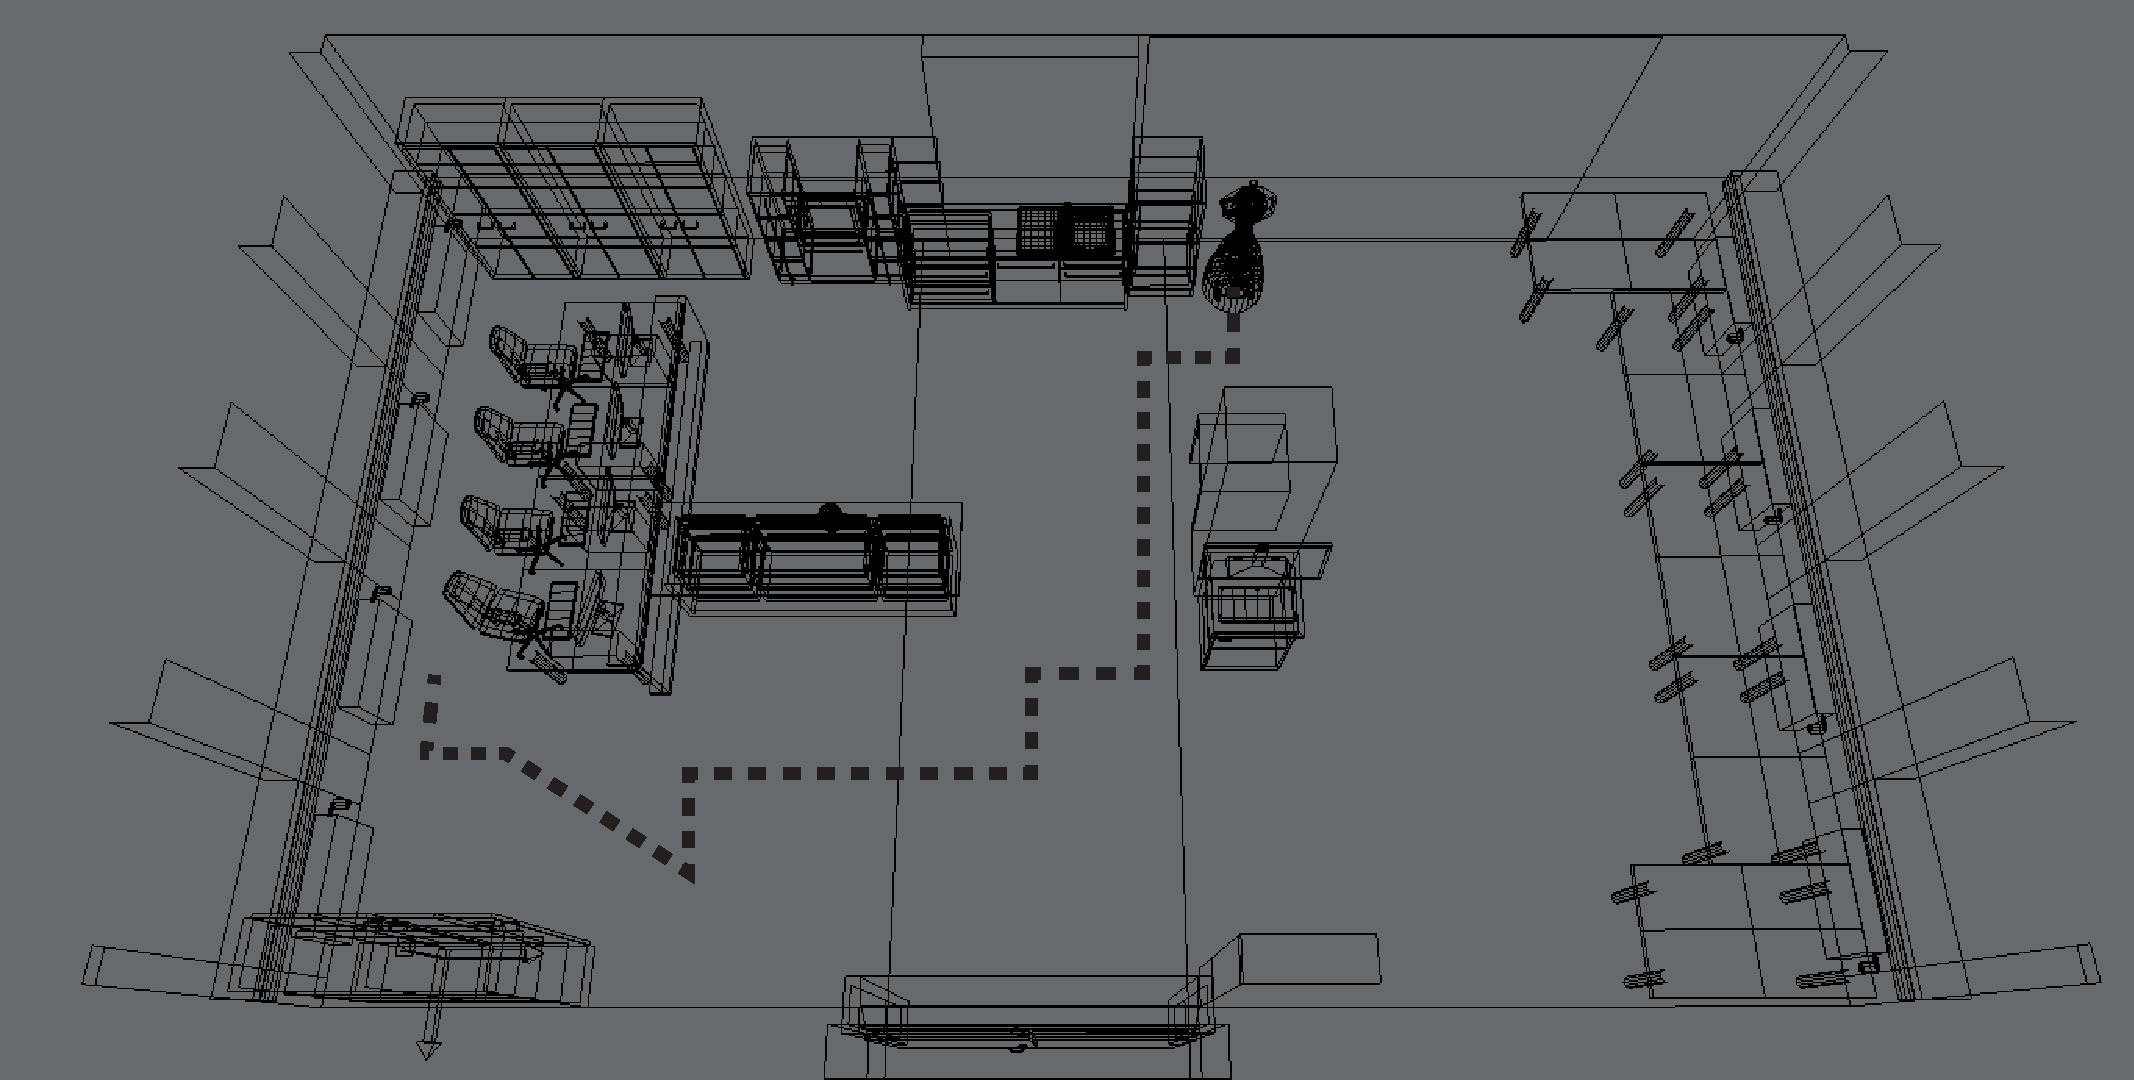
\includegraphics[width=\linewidth]{trajectory_v4}
%		\caption{Trajectory.}
%		\label{fig:demo-trajectory}
%\end{figure}

%\newpage

\section{Experiment Configurations}
\label{sec:scenarios}

\begin{table}[t!]
	\caption{Details on the different configurations used for the experiments on the base (single phase) framework.}
	\label{tab:configurations-base}\centering
	\begin{tabular}{|l|l|r|l|l|r|}
		\hline
		\textbf{ID} & \textbf{Environment} & \textbf{Weight Factor $\beta$} & \textbf{Acquisition Function} & \textbf{Algorithm} & \textbf{Dataset Used} \\
		\hline 
		1 & \texttt{tum\_kitchen} & 0.0 & \acrshort{acr:mei} & $k$-Means & 100\% \\
		\hline
		2 & \texttt{tum\_kitchen} & 0.0 & \acrshort{acr:mei} & $k$-Means & 75\%  \\
		\hline
		3 & \texttt{tum\_kitchen} & 0.0 & \acrshort{acr:mei} & $k$-Means & 50\% \\
		\hline
		4 & \texttt{tum\_kitchen} & 0.0 & \acrshort{acr:gp-ucb} & $k$-Means & 100\% \\
		\hline
		5 & \texttt{tum\_kitchen} & 0.0 & \acrshort{acr:mei-ps} & $k$-Means & 100\% \\
		\hline
		6 & \texttt{tum\_kitchen} & 0.0 & \acrshort{acr:mei} & \acrshort{acr:gmm} & 100\% \\
		\hline
		7 & \texttt{tum\_kitchen} & 0.0 & \acrshort{acr:gp-ucb} & \acrshort{acr:gmm} & 100\% \\
		\hline
		%6 & \texttt{tum\_kitchen} & 0.0 & \acrshort{acr:gp-ucb} & \acrshort{acr:gmm} & 100\% \\
		%\hline
		8 & \texttt{tum\_kitchen} & 0.25 & \acrshort{acr:mei} & $k$-Means & 100\% \\
		\hline
		9 & \texttt{tum\_kitchen} & 0.50 & \acrshort{acr:mei} & $k$-Means & 100\% \\
		\hline
		10 & \texttt{uol\_bl} & 0.0 & \acrshort{acr:mei} & $k$-Means & 100\% \\
		\hline
		%10 & \texttt{uol\_bl} & 0.0 & \acrshort{acr:mei} & $k$-Means & 75\%  \\
		%\hline
		%11 & \texttt{uol\_bl} & 0.0 & \acrshort{acr:mei} & $k$-Means & 50\% \\
		%\hline
		%12 & \texttt{uol\_bl} & 0.0 & \acrshort{acr:mei} & \acrshort{acr:gmm} & 100\% \\
		%\hline
		11 & \texttt{uol\_bl} & 0.0 & \acrshort{acr:gp-ucb} & $k$-Means & 100\% \\
		\hline
		12 & \texttt{uol\_bl} & 0.0 & \acrshort{acr:mei-ps} & $k$-Means & 100\% \\
		\hline
		%14 & \texttt{uol\_bl} & 0.0 & \acrshort{acr:gp-ucb} & \acrshort{acr:gmm} & 100\% \\
		%\hline
		%15 & \texttt{uol\_bl} & 0.25 & \acrshort{acr:mei} & $k$-Means & 100\% \\
		%\hline
		%16 & \texttt{uol\_bl} & 0.50 & \acrshort{acr:mei} & $k$-Means & 100\% \\
		%\hline
	\end{tabular}
\end{table}

\begin{table}[t!]
	\caption{Details on the different configurations used for the experiments on the multi-phase framework.}
	\label{tab:configurations-multi}\centering
	\begin{tabular}{|l|l|r|l|l|r|}
		\hline
		\textbf{ID} & \textbf{Environment} & \textbf{Weight Factor $\beta$} & \textbf{Acquisition Function} & \textbf{Algorithm} & \textbf{Dataset Used} \\
		\hline 
		13 & \texttt{tum\_kitchen} & 0.0 & \acrshort{acr:mei} & $k$-Means & 100\% \\
		\hline
		14 & \texttt{tum\_kitchen} & 0.0 & \acrshort{acr:gp-ucb} & $k$-Means & 100\% \\
		\hline
%		15 & \texttt{tum\_kitchen} & 0.50 & \acrshort{acr:mei} & $k$-Means & 100\% \\
%		\hline
		15 & \texttt{uol\_bl} & 0.0 & \acrshort{acr:mei} & $k$-Means & 100\% \\
		\hline
		16 & \texttt{uol\_bl} & 0.0 & \acrshort{acr:gp-ucb} & $k$-Means & 100\% \\
		\hline
%		17 & \texttt{uol\_bl} & 0.25 & \acrshort{acr:mei} & $k$-Means & 100\% \\
%		\hline
%		18 & \texttt{uol\_bl} & 0.50 & \acrshort{acr:mei} & $k$-Means & 100\% \\
%		\hline
	\end{tabular}
\end{table}

In this section an overview is provided of the experiments that have been performed with the robot navigation implementation of the framework.
\autoref{tab:designer-settings} shows the auxiliary settings used in the experiments for aspects like time-outs, parameter domain and goal radius for each of the environments.
Experiments are conducted for both the \textit{base} framework and \textit{multi-phase} framework with each of the environments.
The configurations for these experiments are shown in \autoref{tab:configurations-base} and \autoref{tab:configurations-multi} respectively.

The configurations were chosen with the aim of being able to identify how the results are affected based on changes in the used acquisition function, weight factor, clustering algorithm and the part of the dataset used.
In each of these experiments data is stored that comprise the generated evidence sets, log-files and the \acrshortpl{acr:mdp} that yield the best performance.
In the next section the obtained results for each of these configurations are shown and discussed accordingly.

%Discuss the different configurations that are to be compared
%\begin{itemize}
%	\item Fixed values for $\beta$-parameter vs. gradually decreasing from $1$ to $0$
%	\item Multiple environments: small (\texttt{tum\_kitchen}); large (\texttt{uol\_bl})
%	\item Model-learning algorithms: direct clustering vs. trajectory clustering; $k$-means vs. GMM
%	\item Data-sets of different sizes
%\end{itemize}

%\noindent Configurations for the basic optimization framework (only based on simulations):
%\begin{itemize}
%	\item Fixed value for $\beta$ (i.e., which weighs $V_\mathit{DTP}$): $0$, $0.25$ and $0.5$
%	\item Acquisition functions: \acrshort{acr:gp-ucb}, \acrshort{acr:mei}
%	\item GMM vs. $k$-Means (vs. trajectory clustering if time available)
%	\item All available data, 75\% and 50\%
%	\item Discount factor: $\gamma = 0.95$
%	\item Small environment: \texttt{tum\_kitchen}; and large environment: \texttt{uol\_bl}
%\end{itemize}
%We need to record: number of iterations, total time passed, optimum found ($\theta_\textnormal{max}$ and $V_{\mathcal{M},\textnormal{max}}$)
%
%\vspace{12pt}
%\noindent For the cost-incremental extension we could try to observe what happens when we decrease $\beta$ gradually over time.
%
%\vspace{12pt}
%\noindent Do we want to do something with `variable resolution' as post-processing step in the experiments?
%
%\vspace{12pt}
%\noindent\fbox{\textbf{TODO:} Table to be added describing the configurations/scenarios for the experiments.}

\section{Results and Discussion}
\label{sec:results}
%vTODO Fix order of figures and update text

From the experiments that have been performed according to the configurations presented in \autoref{sec:scenarios} results have been obtained that are discussed in this section.
First, we present and review the results obtained for the experiments that follow the base framework in \autoref{sec:base-framework-results}.
Then, in \autoref{sec:multiphase-framework-results} the results for the multi-phase extension of the framework are presented and discussed. 
Each of the figures in these sections present plots for each of the experiments, showing the resulting posterior from the gathered evidence, and the value~$V_\mathcal{M}$ of the learned model in each iteration of the \acrshort{acr:bo} optimization process.
%In these plots $\theta$ is the parameter-setting for model learning and $f$ is the (unknown) objective function mapping these to model values.

\subsection{Base Framework}
\label{sec:base-framework-results}

First off, we present and evaluate the results obtained from the experiments on the base framework.
As shown in \autoref{tab:configurations-base}, experiments have been performed on two different simulation environments: the small \texttt{tum\_kitchen} environment and the, in comparison, large \texttt{uol\_bl} environment, for which the results are discussed in the following sections.

\begin{figure}[t]
	\centering
	\captionsetup{font=small}
	\captionsetup[subfigure]{font=footnotesize}
	\captionsetup[subfigure]{justification=centering}
	\begin{subfigure}[t]{0.495\textwidth}
		\includegraphics[width=\textwidth]{plots/tum_base/plot_b_00__alg_kmeans_pct_100_acq_ei}
		\caption{Experiment 1: 100\% of the dataset used}
		\label{fig:exp1}
	\end{subfigure}
	\begin{subfigure}[t]{0.495\textwidth}
		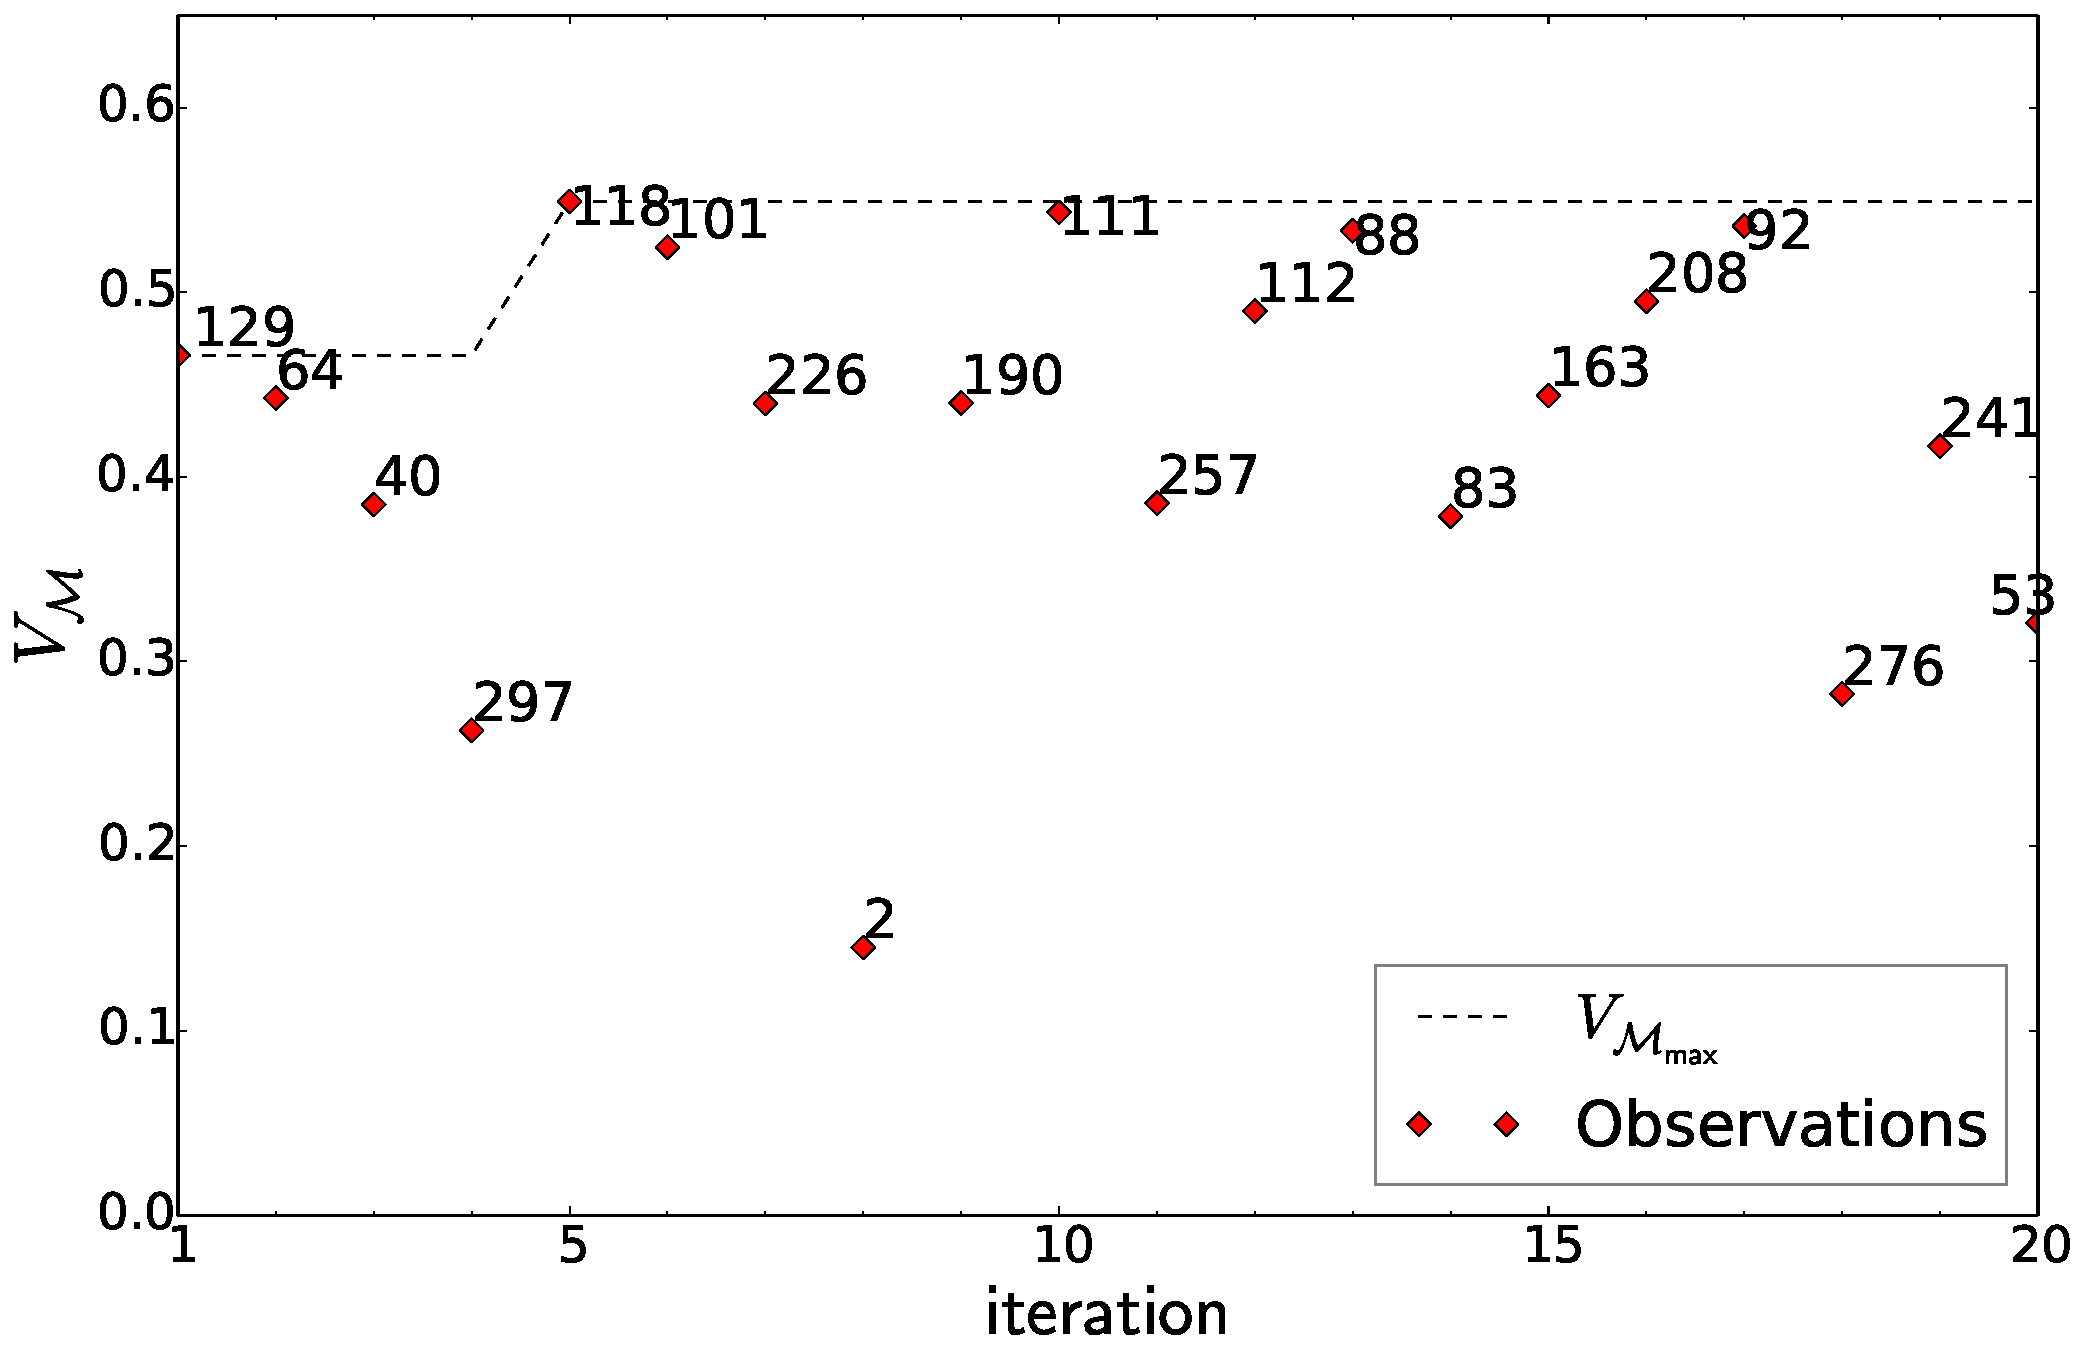
\includegraphics[width=\textwidth]{plots/tum_base/plot_b_00__alg_kmeans_pct_100_acq_ei_maximum_2}
		\caption{Experiment 1: Observations over iterations}
		\label{fig:exp1_observations}
	\end{subfigure}
	\begin{subfigure}[t]{0.495\textwidth}
		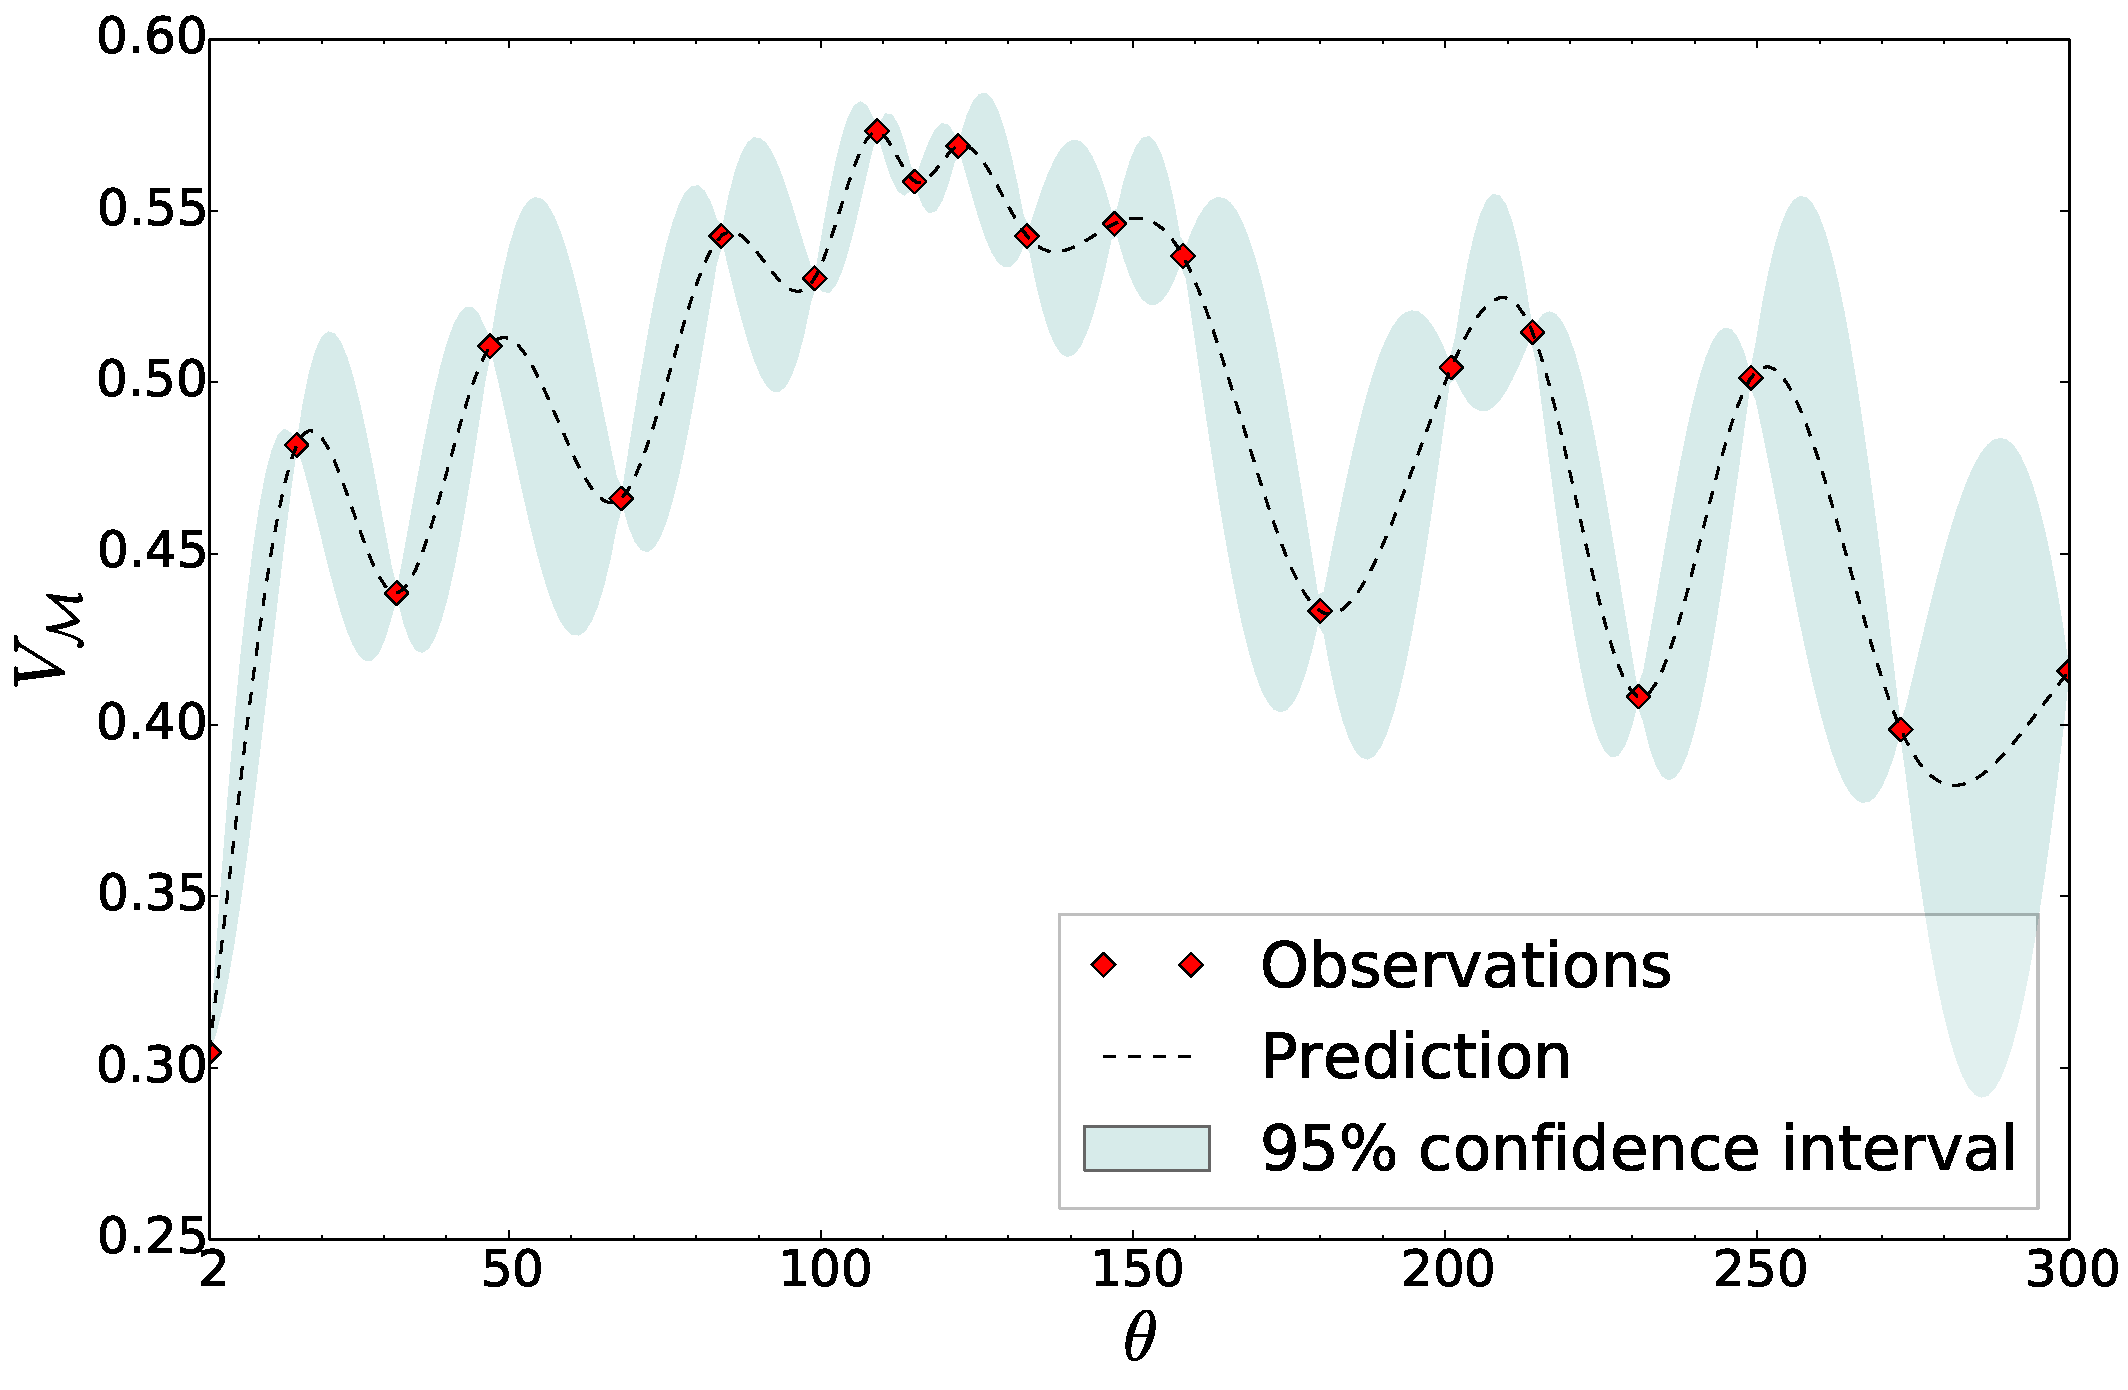
\includegraphics[width=\textwidth]{plots/tum_base/plot_b_00__alg_kmeans_pct_75_acq_ei}
		\caption{Experiment 2: 75\% of the dataset used}
		\label{fig:exp2}
	\end{subfigure}
	\begin{subfigure}[t]{0.495\textwidth}
		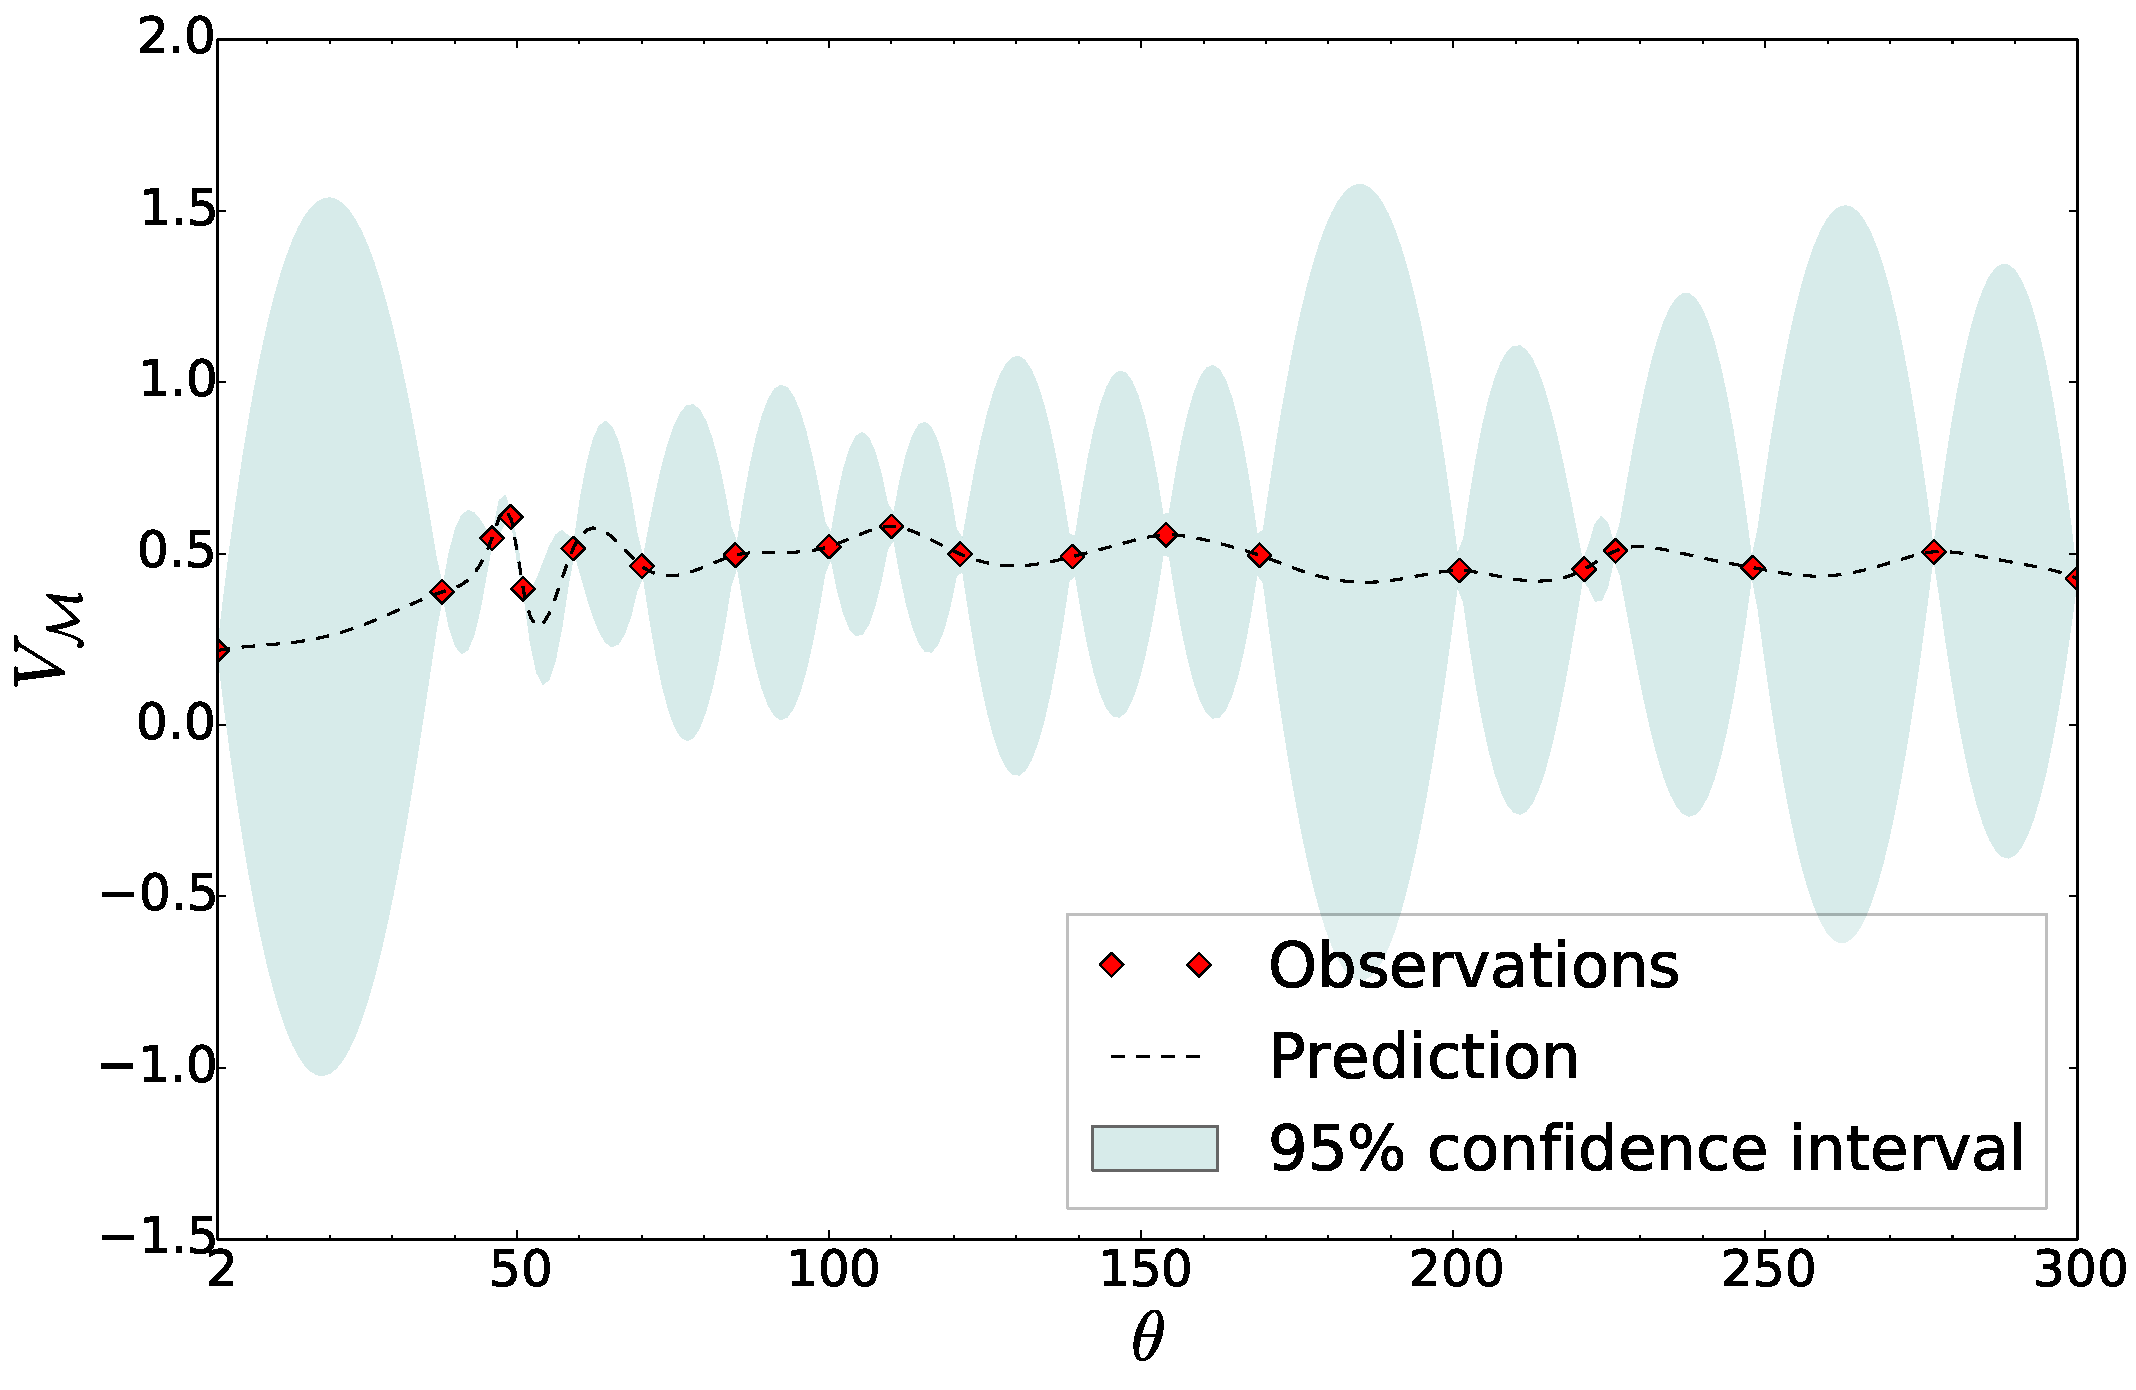
\includegraphics[width=\textwidth]{plots/tum_base/plot_b_00__alg_kmeans_pct_50_acq_ei}
		\caption{Experiment 3: 50\% of the dataset used}
		\label{fig:exp3}
	\end{subfigure}
	\caption{Plots showing a comparison of the resulting \acrshort{acr:gp} posterior for different dataset sizes. The plots correspond to 20 iterations of the base framework on the \texttt{tum\_kitchen} environment with $\beta = 0.0$, $k$-Means clustering and \acrshort{acr:mei} acquisition function used.}
	\label{fig:plots_tum_base_data}
\end{figure}

\subsubsection{Tum Kitchen Environment}

First of all, let us consider the results obtained for the small \texttt{tum\_kitchen} environment.
Overall, in \Crefrange{fig:plots_tum_base_acq}{fig:plots_tum_base_weight} one can see that the optimum $\theta_\mathsf{max}$ is mostly found within similar areas of the parameter space $\Theta$.
In \autoref{fig:plots_tum_base_data} we compare the effect of using different dataset sizes for learning \acrshortpl{acr:mdp}.
In \autoref{fig:exp1}, \autoref{fig:exp2} and \autoref{fig:exp3} the resulting \acrshort{acr:gp} is shown after respectively using 100\%, 75\% and 50\% of the dataset in the corresponding experiments.
One can see in \autoref{fig:exp3} that with 50\% of the data employed, the observed model values~$V_\mathcal{M}$ for different settings of $\theta$ involve quite some noise.
In this figure one can also see that the \acrshort{acr:gp} is quite sensitive to this noise and accordingly over-fits on these observations, so that the uncertainty about the parameter space is quite large.
At the other hand, \autoref{fig:exp2} shows that with 75\% of the data the distinction becomes much more clear, even though the higher variance is still present, particularly for larger settings of $\theta$.
This clearly shows that sufficient data is needed to avoid overfitting and obtaining more stable results with discernible performance measures.

%What might explain this, is that this particular section of the dataset adds data based on which \acrshortpl{acr:mdp} with large state spaces overfit their corresponding transition function.

\begin{figure}[t]
	\centering
	\captionsetup{font=small}
	\captionsetup[subfigure]{font=footnotesize}
	\captionsetup[subfigure]{justification=centering}
	\begin{subfigure}[t]{0.495\textwidth}
		\includegraphics[width=\textwidth]{plots/tum_base/plot_b_00__alg_kmeans_pct_100_acq_ucb}
		\caption{Experiment 4: \acrshort{acr:gp-ucb} acquisition function used}
		\label{fig:exp4}
	\end{subfigure}
	\begin{subfigure}[t]{0.495\textwidth}
		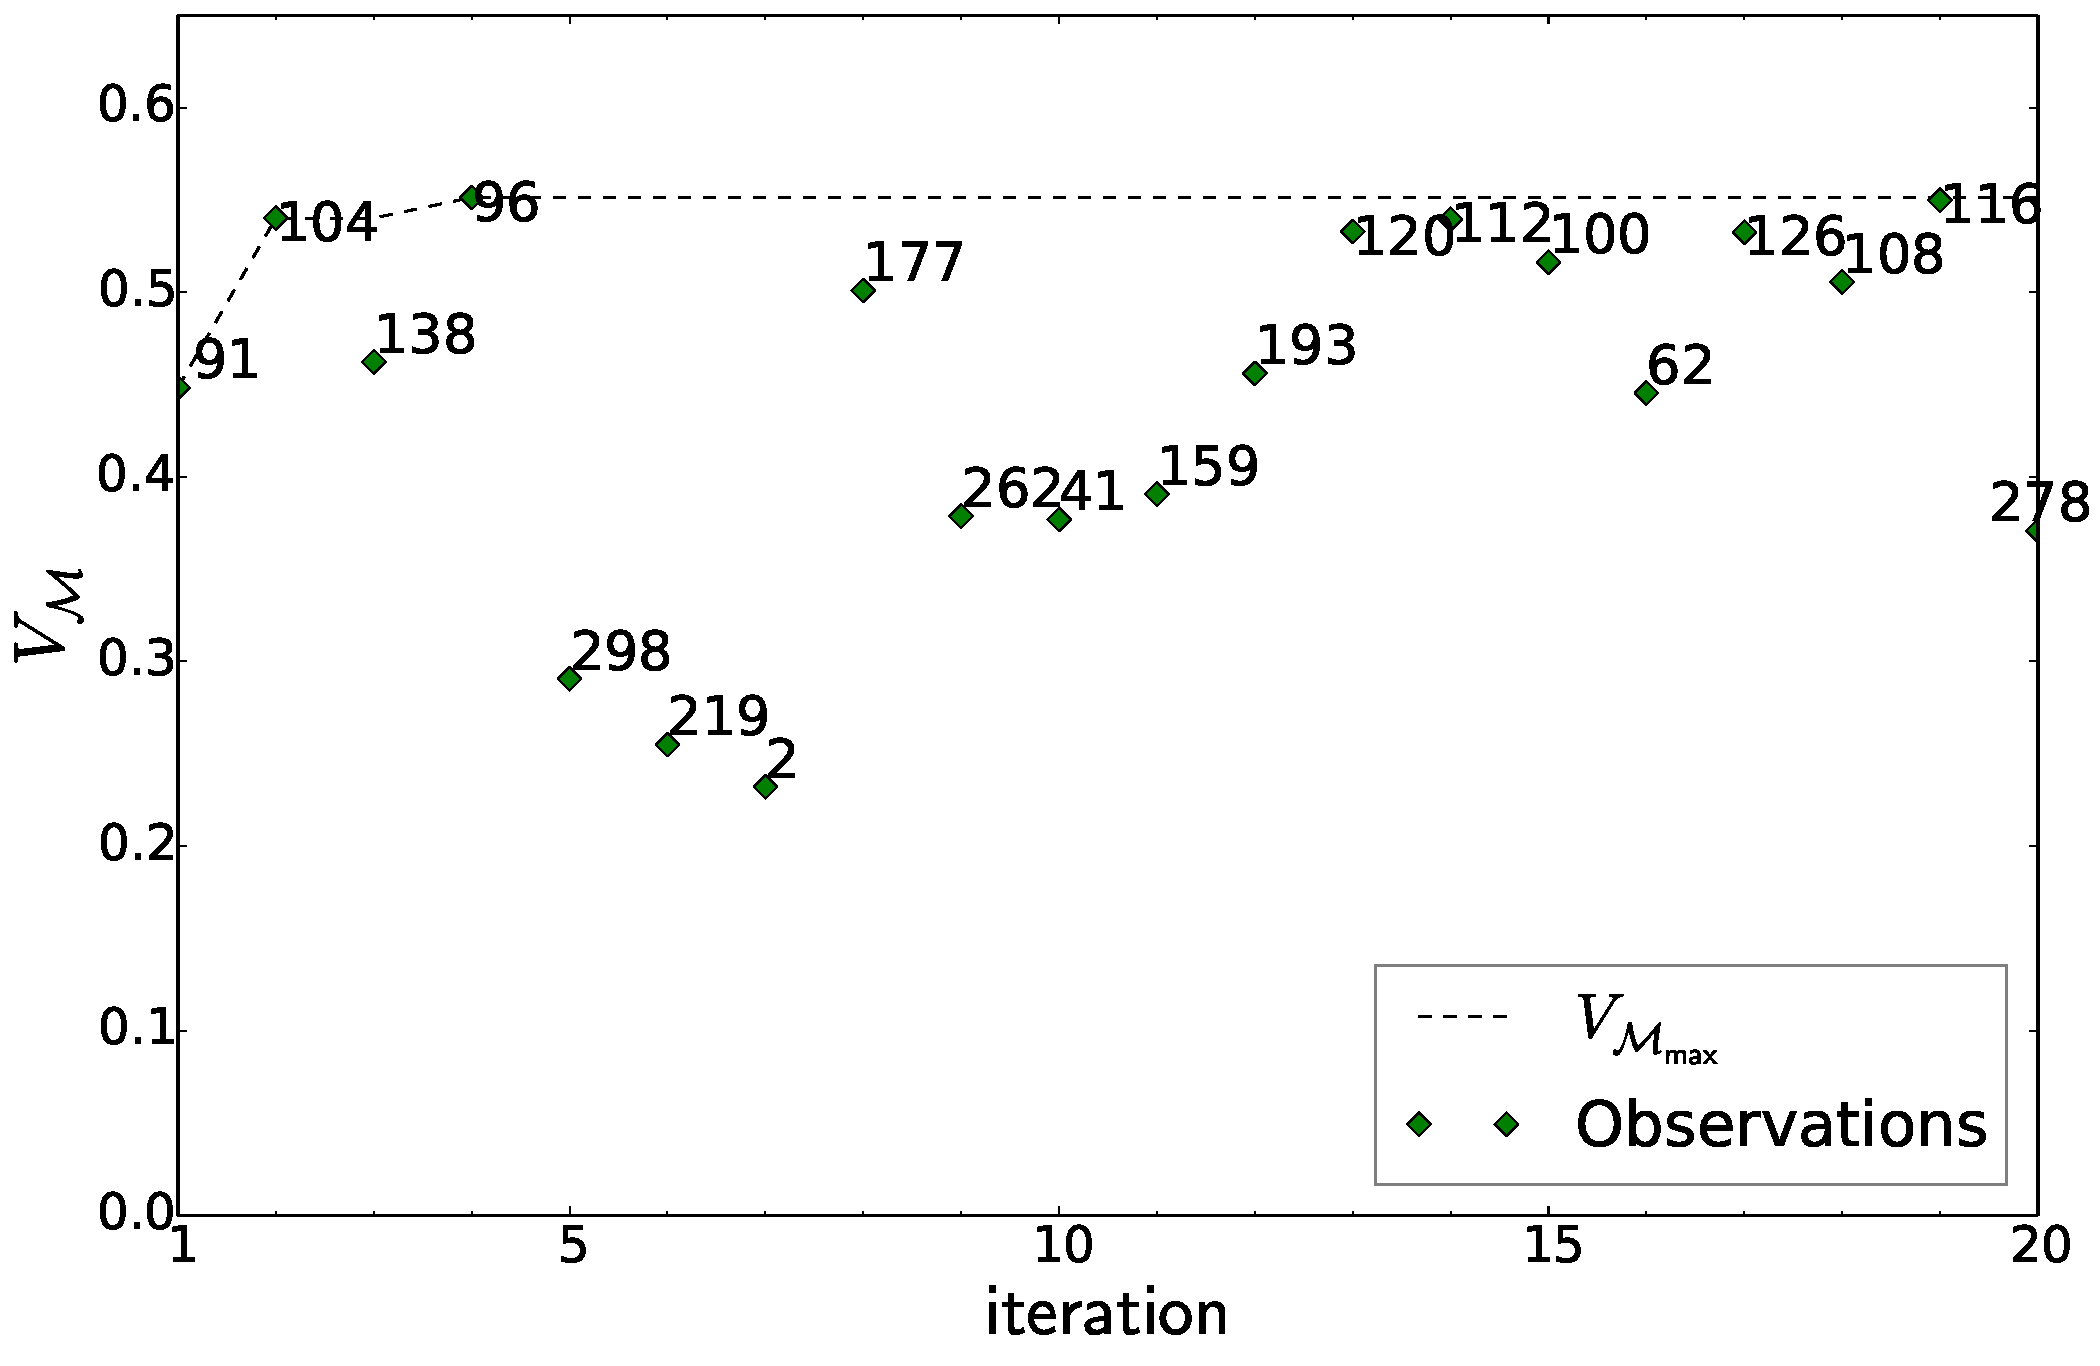
\includegraphics[width=\textwidth]{plots/tum_base/plot_b_00__alg_kmeans_pct_100_acq_ucb_maximum_2}
		\caption{Experiment 4: Observations over iterations}
		\label{fig:exp4_observations}
	\end{subfigure}
	\begin{subfigure}[t]{0.495\textwidth}
		\includegraphics[width=\textwidth]{plots/tum_base/plot_b_00__alg_kmeans_pct_100_acq_eips}
		\caption{Experiment 5: \acrshort{acr:mei-ps} acquisition function used}
		\label{fig:exp5}
	\end{subfigure}
	\begin{subfigure}[t]{0.495\textwidth}
		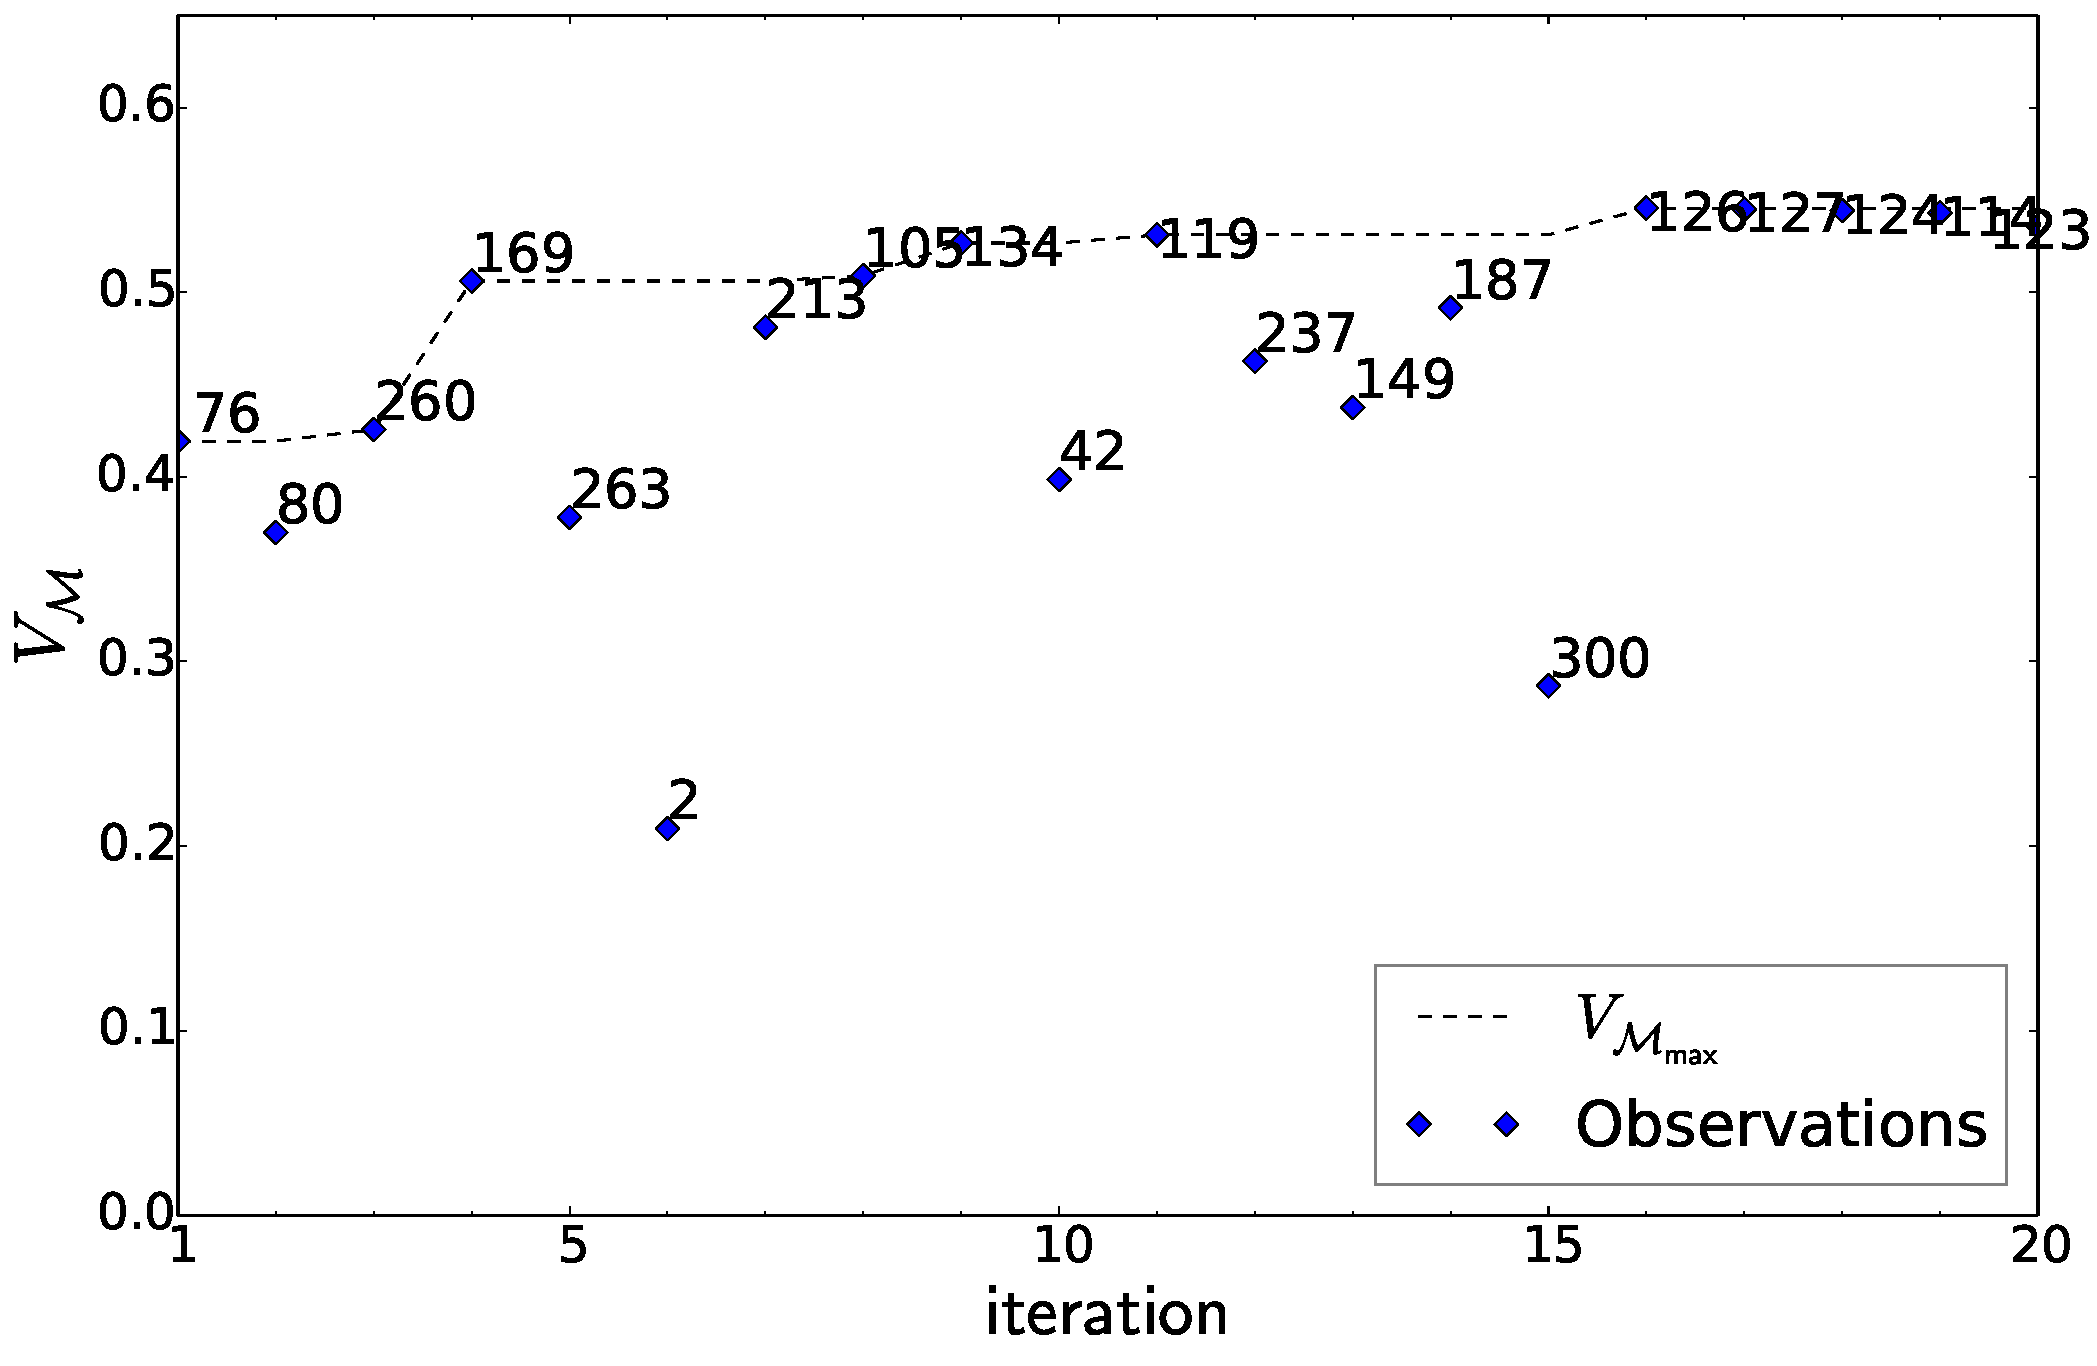
\includegraphics[width=\textwidth]{plots/tum_base/plot_b_00__alg_kmeans_pct_100_acq_eips_maximum_2}
		\caption{Experiment 5: Observations over iterations}
		\label{fig:exp5_observations}
	\end{subfigure}
	\caption{Plots showing a comparison of the resulting \acrshort{acr:gp} posterior for varying acquisition functions. The plots correspond to 20 iterations of the base framework on the \texttt{tum\_kitchen} environment with $\beta = 0.0$ and $k$-Means~clustering used.}
	\label{fig:plots_tum_base_acq}
\end{figure}

\begin{figure}[t!]
	\centering
	\captionsetup{font=small}
	\captionsetup[subfigure]{font=footnotesize}
	\captionsetup[subfigure]{justification=centering}
	\begin{subfigure}[t]{0.495\textwidth}
		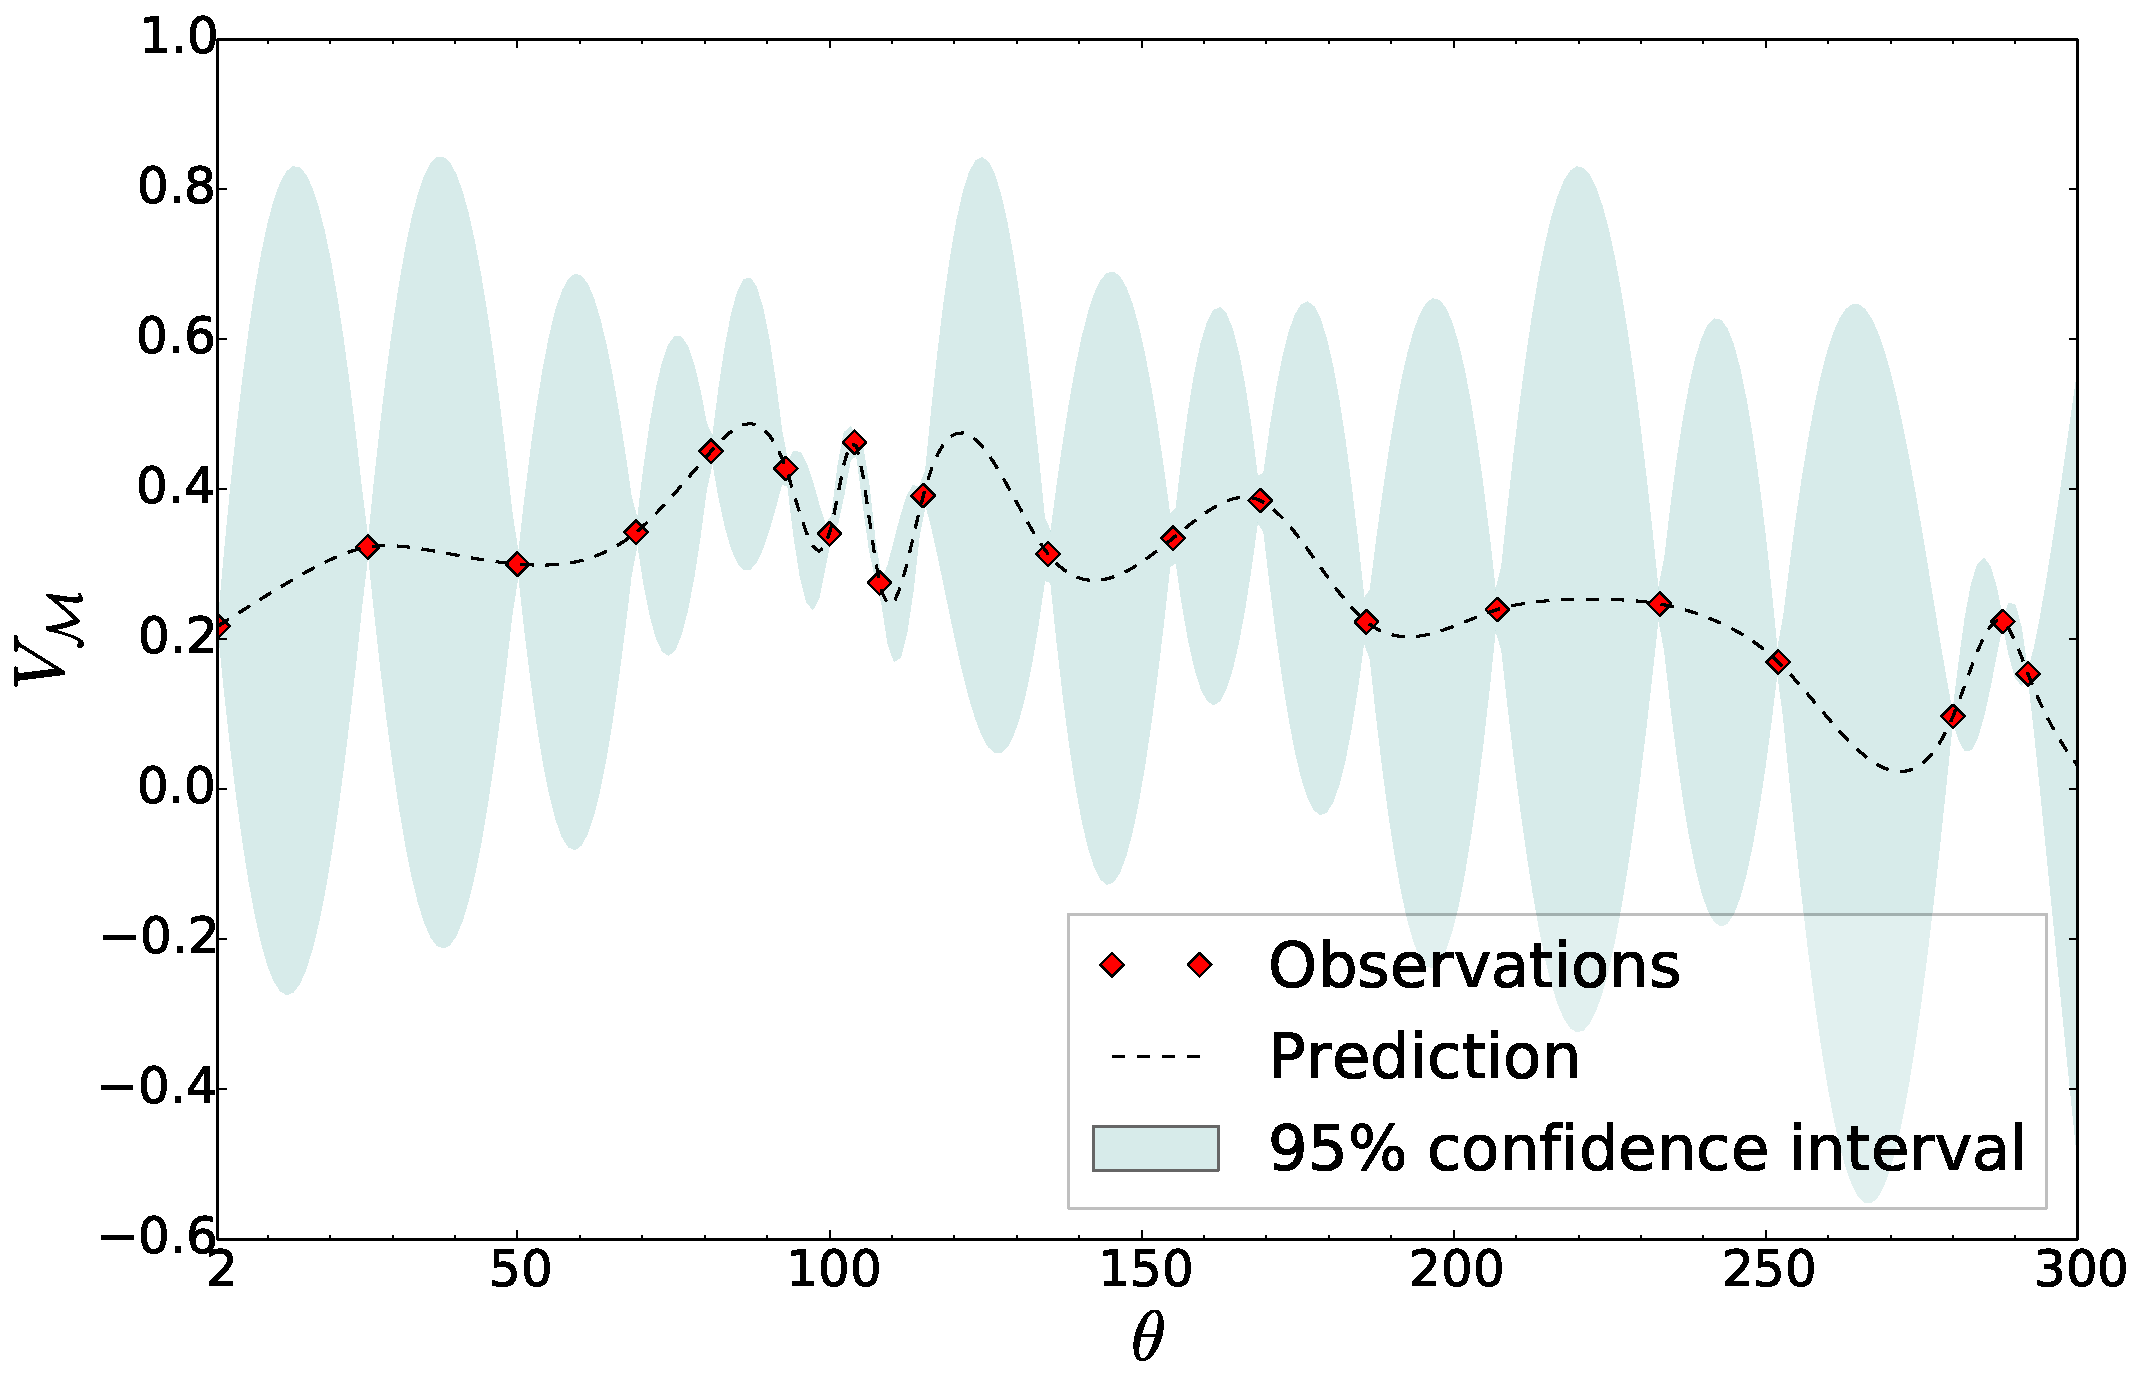
\includegraphics[width=\textwidth]{plots/tum_base/plot_b_00__alg_gmm_pct_100_acq_ei}
		\caption{Experiment 6: \acrshort{acr:mei} acquisition function used}
		\label{fig:exp6}
	\end{subfigure}
	\begin{subfigure}[t]{0.495\textwidth}
		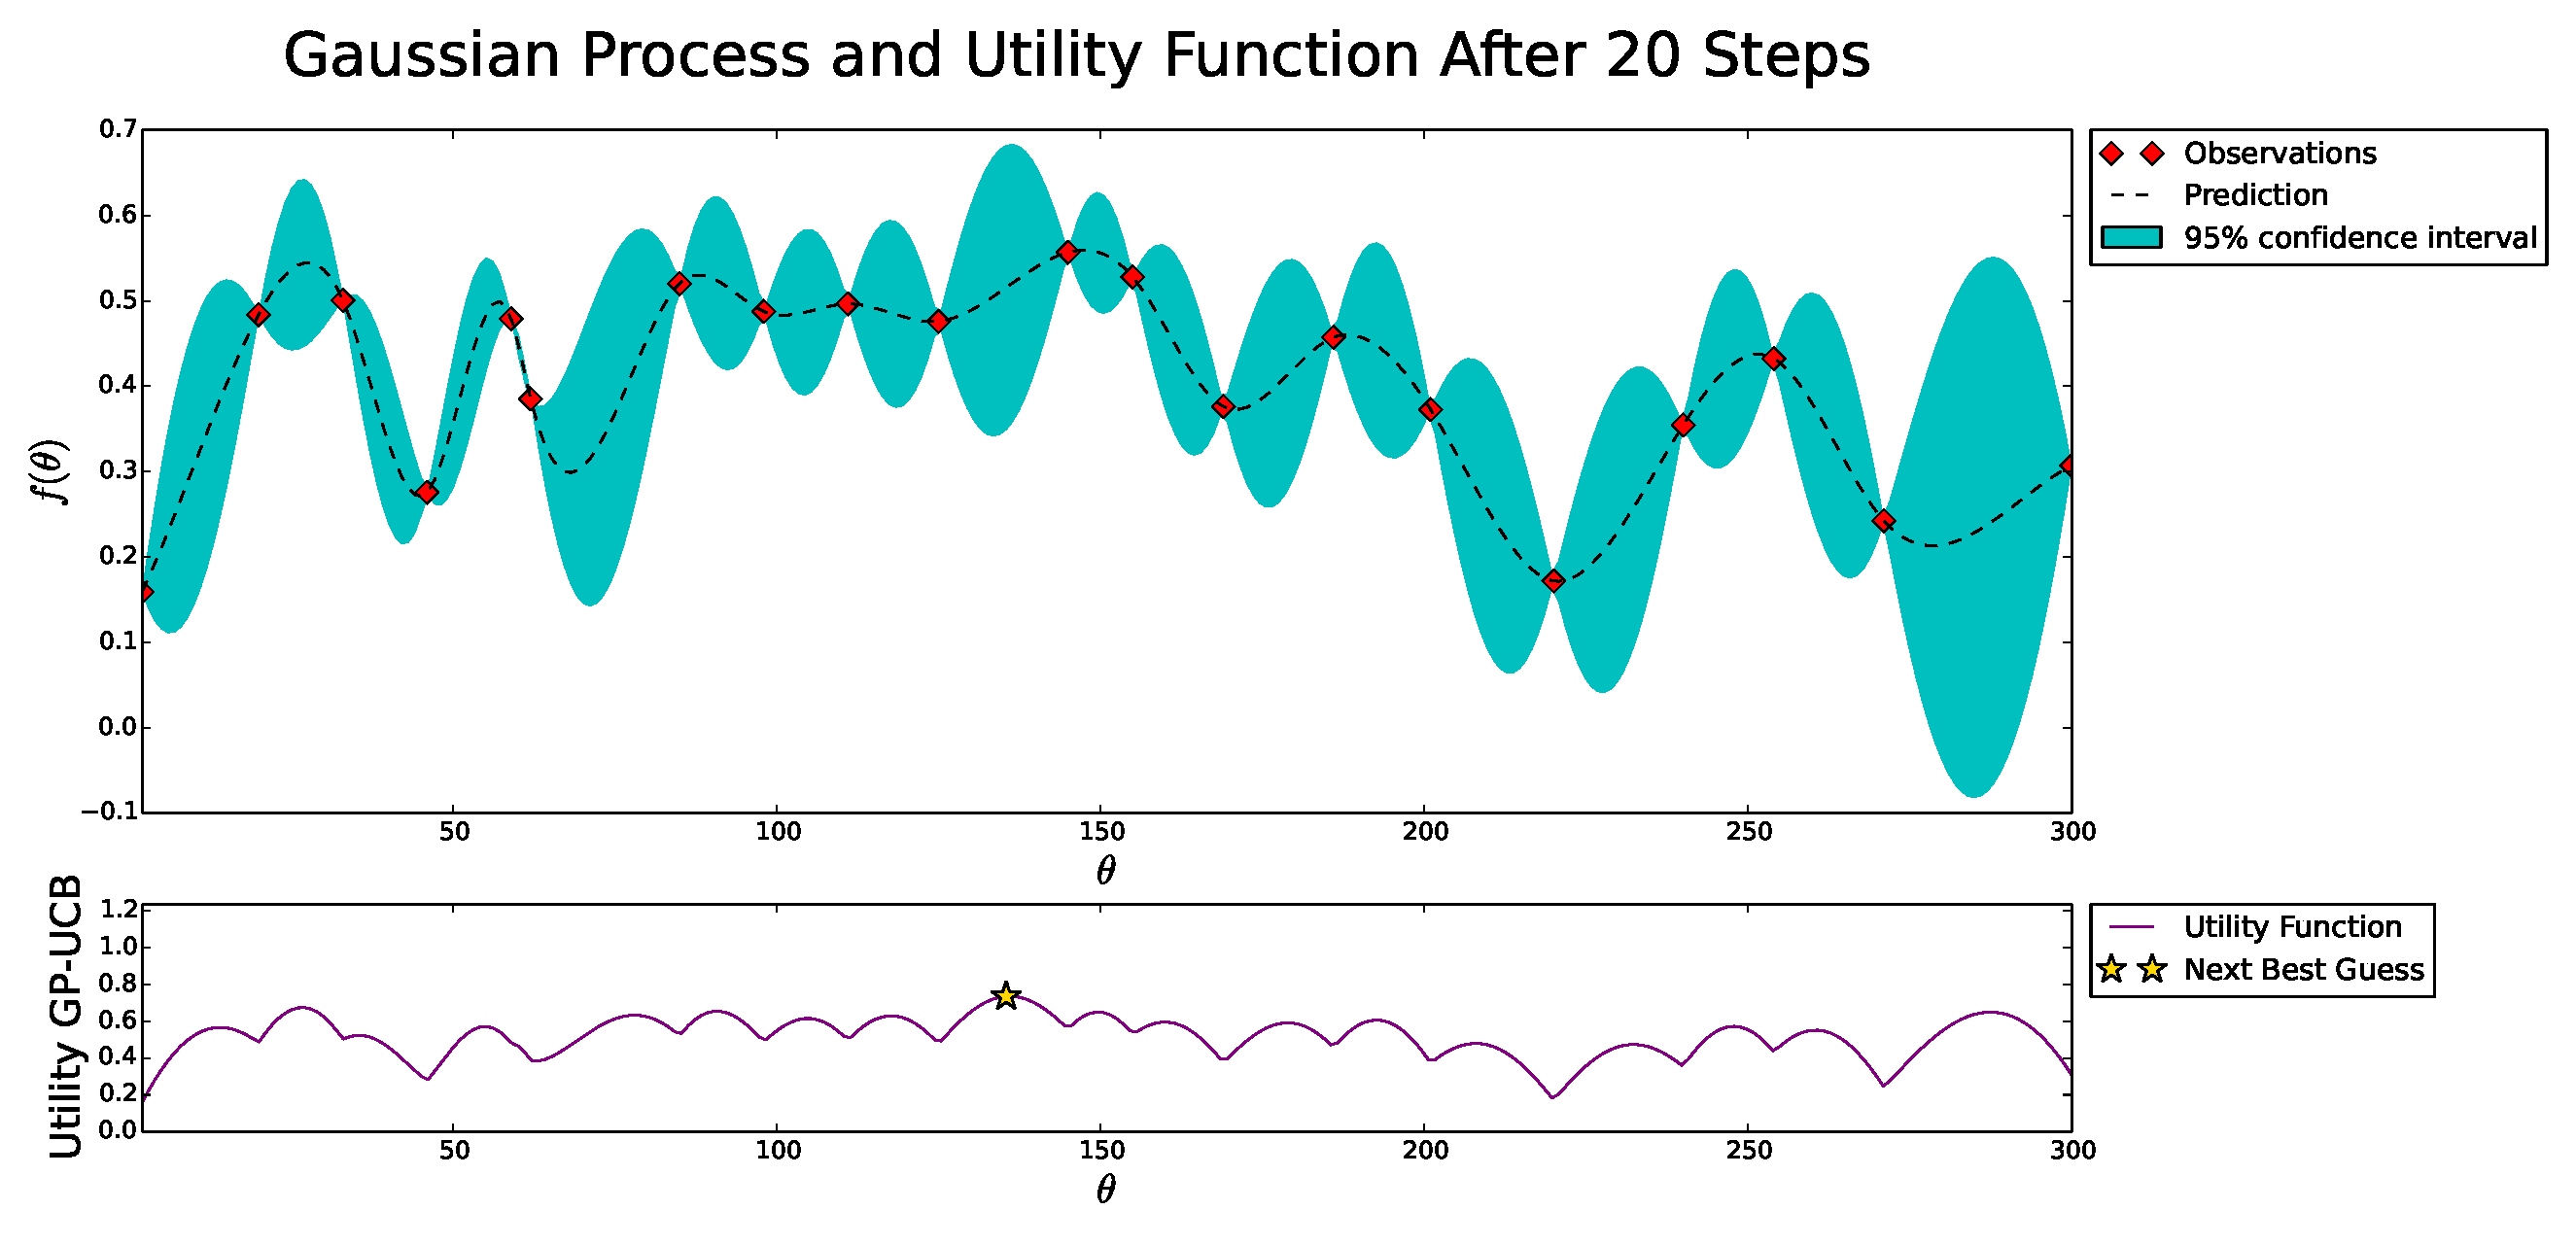
\includegraphics[width=\textwidth]{plots/tum_base/plot_b_00__alg_gmm_pct_100_acq_ucb}
		\caption{Experiment 7: \acrshort{acr:gp-ucb} acquisition function used}
		\label{fig:exp7}
	\end{subfigure}
	\caption{Plots showing a comparison of the resulting \acrshort{acr:gp} posterior for varying acquisition functions. The plots correspond to 20 iterations of the base framework on the \texttt{tum\_kitchen} environment with $\beta = 0.0$ and \acrshort{acr:gmm}~used.}
	\label{fig:plots_tum_base_gmm}
\end{figure}

\newpage

Next, let us compare the results depicted in \autoref{fig:exp1} and \autoref{fig:plots_tum_base_acq} where different acquisition functions are used in the \acrshort{acr:bo} framework (i.e., \acrshort{acr:mei}, \acrshort{acr:gp-ucb} and \acrshort{acr:mei-ps} respectively).
In addition, we present some plots that show how the different acquisition function samples new observations in \autoref{fig:exp1_observations}, \autoref{fig:exp4_observations} and \autoref{fig:exp5_observations}.

First of all, we see that in each of these experiments a global maximum is found in the same area of the parameter space.
%For this environment, we see the results are quite similar, and also in the logs made from the experiments it was seen that the maximum observation was done in the (exact) same number of steps (in the third step).
%The most clear difference is seen in the `behavior' of the \acrshort{acr:gp-ucb} acquisition function, being optimistic in the face of uncertainty, so that the confidence intervals are restricted for promising areas of the parameter space.
%On the other hand, the influence of the timing \acrshort{acr:gp} in the \acrshort{acr:mei-ps} acquisition  is absent for our experiments in the \texttt{tum\_kitchen} environment, as the difference in the required time for model learning and planning is minimal.
For this environment the \acrshort{acr:gp-ucb} and \acrshort{acr:mei-ps} lead to a more clear convergence to the area of the parameter space with the global optimum.
The benefits of the timing \acrshort{acr:gp} in the \acrshort{acr:mei-ps} is only limited for this environment as the time for model learning and planning are closer together than for the \texttt{uol\_bl} environment.

Then, in \autoref{fig:exp6} and \autoref{fig:exp7} we see the plots for the experiments in which instead \acrshortpl{acr:gmm} are used for learning state spaces for our \acrshortpl{acr:mdp}.
We observe that again for this algorithm, the optima are found within the same areas of the parameter space for both experiments with different acquisition functions.
The main thing we observe is that, the observed model values $V_\mathcal{M}$ is overall lower with the \acrshort{acr:gmm} employed in comparison to the values observed with $k$-Means employed.
Therefore, employing $k$-Means appears more suitable to learn the state space for \acrshortpl{acr:mdp} in our application of mobile robot navigation.

\begin{figure}[!t]
	\centering
	\captionsetup{font=small}
	\captionsetup[subfigure]{font=footnotesize}
	\captionsetup[subfigure]{justification=centering}
	\begin{subfigure}[t]{0.495\textwidth}
		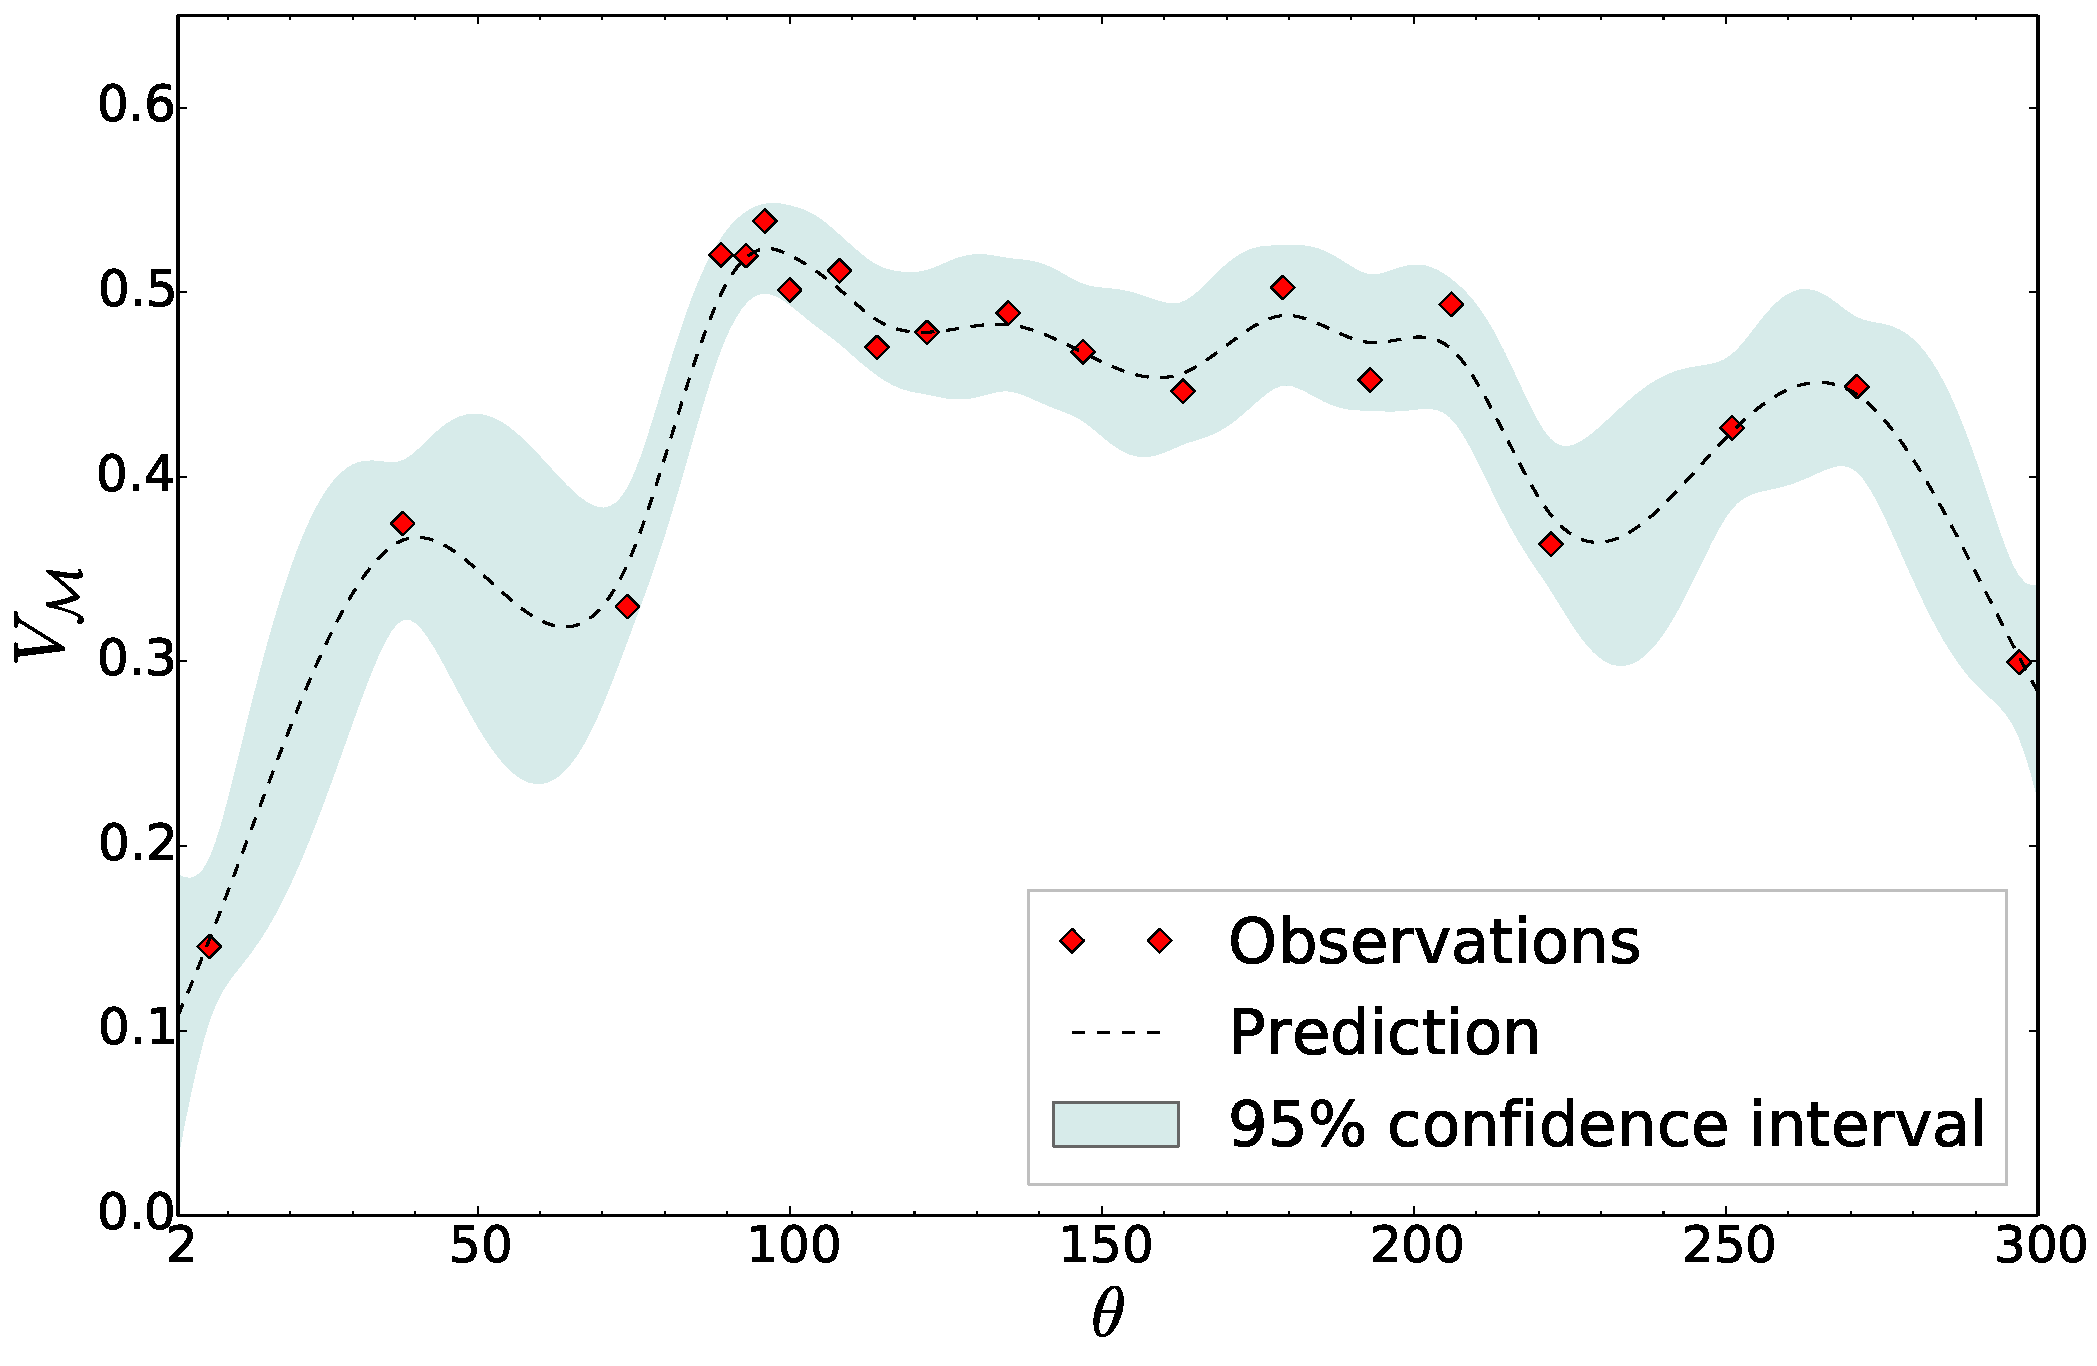
\includegraphics[width=\textwidth]{plots/tum_base/plot_b_025__alg_kmeans_pct_100_acq_ei}
		\caption{Experiment 8: Weight factor $\beta = 0.25$}
		\label{fig:exp8}
	\end{subfigure}
	\begin{subfigure}[t]{0.495\textwidth}
		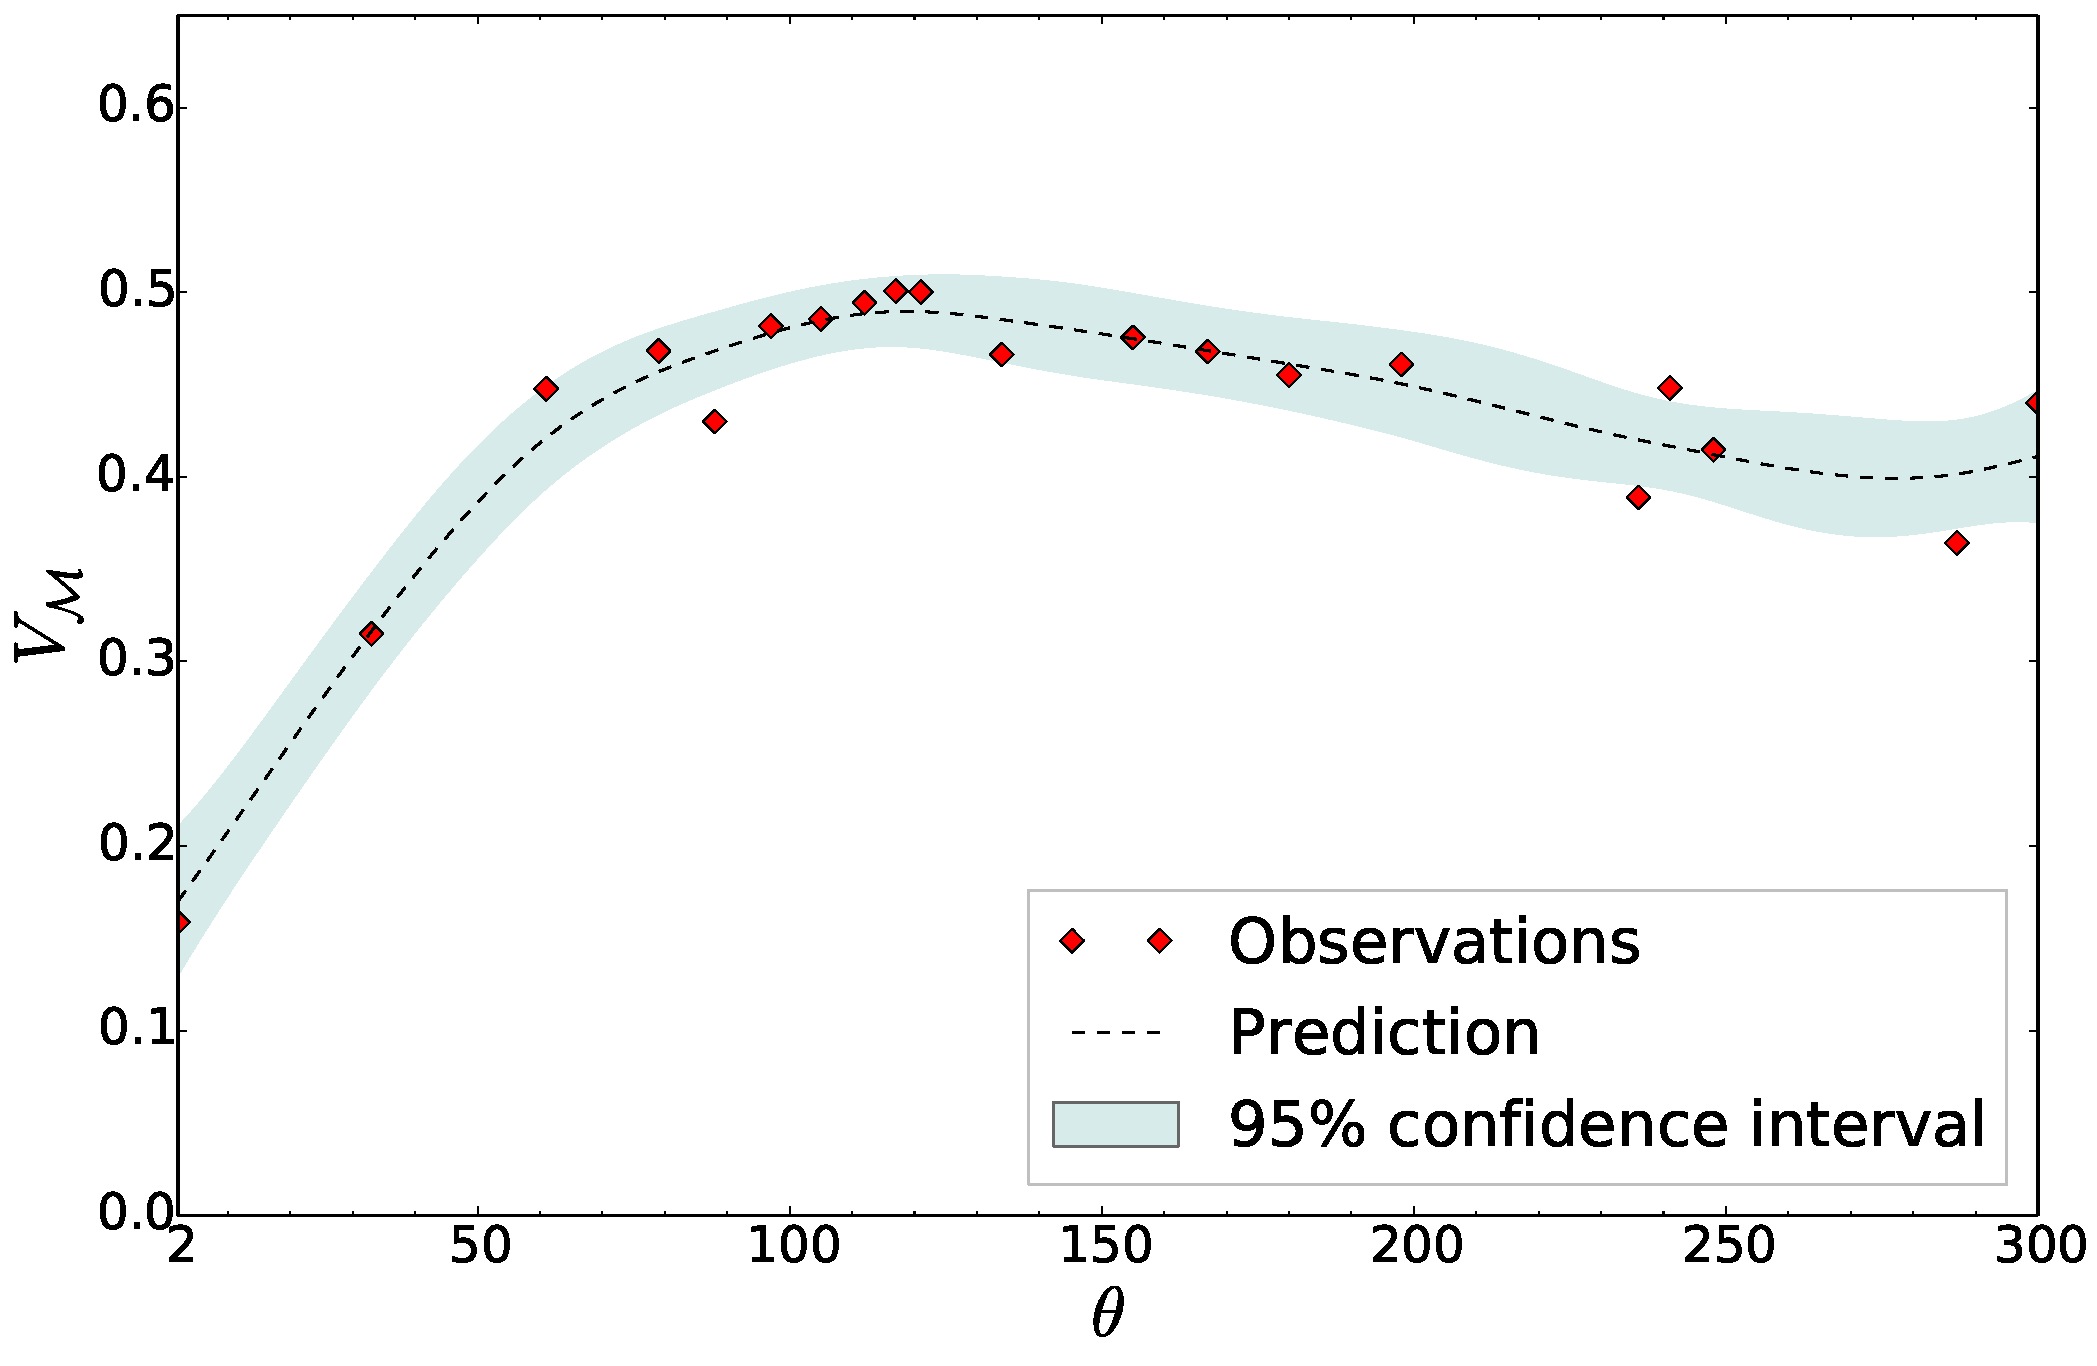
\includegraphics[width=\textwidth]{plots/tum_base/plot_b_05__alg_kmeans_pct_100_acq_ei}
		\caption{Experiment 9: Weight factor $\beta = 0.5$}
		\label{fig:exp9}
	\end{subfigure}
	\caption{Plots showing a comparison of the resulting \acrshort{acr:gp} posterior for varying settings of the $\beta$ factor. The plots correspond to 20 iterations of the base framework on the \texttt{tum\_kitchen} environment with $k$-Means clustering and \acrshort{acr:mei} acquisition used.}
	\label{fig:plots_tum_base_weight}
\end{figure}
	
Finally, we look at the influence of the weight factor $\beta$ for the small environment considering the plots of \autoref{fig:exp1}, \autoref{fig:exp8} and \autoref{fig:exp9}.
In this particular situation, one might benefit from weighing $V_\mathit{DTP}$ in the model value, as it could make a clearer distinction between values for different settings of $\theta$, because it cancels out part of the uncertainty from the simulations.
The intuition of why this works well for this particular environment can be elucidated by \autoref{fig:plots_tum_multi_acq}, which shows that the maxima of the $V_\mathit{DTP}$ and $V_\mathit{SIM}$ measures lie close together.
However, setting $\beta > 0$ might also lead to a bias in other environments, which is that, although $V_\mathit{DTP}$ may have high value, computed policies may not work well in the simulations or the real world.

\subsubsection{UOL BL Environment}

Let us next consider the results for the large \texttt{uol\_bl} environment. In \autoref{fig:plots_uol_base_acq} plots are shown for the experiments in which different acquisitions were used in the \acrshort{acr:bo}.
One can observe the optima found in each of these experiments lie close together.
The experiment that employs the \acrshort{acr:mei} function, however, appears ineffective to find the same global maximum in multiple repetitions.
All in all, the \acrshort{acr:gp-ucb} and especially the \acrshort{acr:mei-ps} function appear most effective in sampling parameter settings that result in \acrshortpl{acr:mdp} yielding high performance.

\afterpage{
\begin{figure}[!t]
	\centering
	\captionsetup{font=small}
	\captionsetup[subfigure]{font=footnotesize}
	\captionsetup[subfigure]{justification=centering}
	\begin{subfigure}[t]{0.65\textwidth}
		\includegraphics[width=\textwidth]{plots/uol_base/plot_b_00__alg_kmeans_pct_100_acq_ei}
		\caption{Experiment 10: \acrshort{acr:mei} acquisition function used}
		\label{fig:exp10}
	\end{subfigure}
	\bigskip
	
	\begin{subfigure}[t]{0.65\textwidth}
		\includegraphics[width=\textwidth]{plots/uol_base/plot_b_00__alg_kmeans_pct_100_acq_ucb}
		\caption{Experiment 11: \acrshort{acr:gp-ucb} acquisition function used}
		\label{fig:exp11}
	\end{subfigure}
	\bigskip
	
	\begin{subfigure}[t]{0.65\textwidth}
		\includegraphics[width=\textwidth]{plots/uol_base/plot_b_00__alg_kmeans_pct_100_acq_eips}
		\caption{Experiment 12: \acrshort{acr:mei-ps} acquisition function used}
		\label{fig:exp12}
	\end{subfigure}
	\bigskip
	\caption{Plots showing a comparison of the resulting \acrshort{acr:gp} posterior for varying acquisition functions. The plots correspond to the \texttt{uol\_bl} environment with $\beta = 0.0$ and $k$-Means~clustering~used.}
	\label{fig:plots_uol_base_acq}
\end{figure}
\clearpage
}

\newpage

\begin{figure}[!t]
	\centering
	\captionsetup{font=small}
	\captionsetup[subfigure]{font=footnotesize}
	\captionsetup[subfigure]{justification=centering}
	\begin{subfigure}[t]{0.495\textwidth}
		\includegraphics[width=\textwidth]{plots/tum_multi/plot_b_00__alg_kmeans_pct_100_acq_ei}
		\caption{Experiment 13: \acrshort{acr:mei} acquisition function in phase 1}
		\label{fig:exp13}
	\end{subfigure}
	\begin{subfigure}[t]{0.495\textwidth}
		\includegraphics[width=\textwidth]{plots/tum_multi/plot_b_00__alg_kmeans_pct_100_acq_ucb}
		\caption{Experiment 14: \acrshort{acr:gp-ucb} acquisition function in phase 1}
		\label{fig:exp14}
	\end{subfigure}
	\caption{Plots showing a comparison of the resulting \acrshort{acr:gp} posterior for varying acquisition functions. The plots correspond to 20 iterations of the multi-phase framework on the \texttt{tum\_kitchen} environment with $\beta = 0.0$ and $k$-Means~clustering~used.}
	\label{fig:plots_tum_multi_acq}
	
	\null
	\begin{subfigure}[t]{0.495\textwidth}
		\includegraphics[width=\textwidth]{plots/uol_multi/plot_b_00__alg_kmeans_pct_100_acq_ei}
		\caption{Experiment 15: \acrshort{acr:mei} acquisition function in phase 1}
		\label{fig:exp15}
	\end{subfigure}
	\begin{subfigure}[t]{0.495\textwidth}
		\includegraphics[width=\textwidth]{plots/uol_multi/plot_b_00__alg_kmeans_pct_100_acq_ucb}
		\caption{Experiment 16: \acrshort{acr:gp-ucb} acquisition function in phase 1}
		\label{fig:exp16}
	\end{subfigure}
	\caption{Plots showing a comparison of the resulting \acrshort{acr:gp} posterior for varying acquisition functions. The plots correspond to 30 iterations of the multi-phase framework on the \texttt{uol\_bl} environment with $\beta = 0.0$ and $k$-Means~clustering~used.}
	\label{fig:plots_uol_multi_acq}
\end{figure}

\begin{table}[t!]
	\centering
	\caption{Overview of the time expenses of a single iteration for model learning, planning and simulation with the algorithms used in the experiments. The time expenses are presented as ranges for the smallest and largest \acrshortpl{acr:mdp} learned for the environment.}
	\label{tab:framework-time-expenses}
	\begin{tabular}{|l|r|r|r|}
		\hline
		\textbf{Environment}    & \textbf{Model Learning Time (\si{\second})} & \textbf{Planning Time (\si{\second})} & \textbf{Simulation Time (\si{\second})} \\ \hline
		\texttt{tum\_kitchen} & \numrange[range-phrase = --]{0.2}{15.0}       & \numrange[range-phrase = --]{0.01}{0.5} & \numrange[range-phrase = --]{110}{200}                         \\ \hline
		\texttt{uol\_bl}      & \numrange[range-phrase = --]{1.0}{60.0}       & \numrange[range-phrase = --]{0.05}{5.0}   & \numrange[range-phrase = --]{100}{700}                        \\ \hline
	\end{tabular}
\end{table}

\subsection{Multi-Phase Framework}
\label{sec:multiphase-framework-results}

%In \Crefrange{fig:exp13}{fig:exp16} one can see that optima are found within the same area of the parameter space as seen in the results for the base framework.
Next, we present and evaluate our results obtained in the experiments on the multi-phase framework, for which the configurations are presented in \autoref{tab:configurations-multi}.
In these experiments, first an optimization takes place of the model value computed solely from the value functions for the tasks the system is expected perform.
Only computing the value functions for \acrshortpl{acr:mdp} as is done in this first phase is relatively time-cheap (i.e., a matter of minutes) in comparison to performing time-costly simulations (i.e., taking multiple hours) as is done in the second phase.
In \autoref{tab:framework-time-expenses} we present an overview to give an idea of the difference in time expenses between learning \acrshort{acr:mdp}, running \acrshort{acr:vi} to compute plans, and running simulations in the Morse simulator.
In the plots in \Crefrange{fig:exp13}{fig:exp16}, the prediction mean resulting from this first phase is depicted by a dotted line.
In the second phase, the posterior from the first phase is utilized to steer the acquisition of the first few samples as described in \autoref{sec:multi-phase-framework}.
The~\acrshort{acr:bo} in both of these phases is preceded by collecting a set of $5$ random samples.
%Our hypothesis is that using the \acrshort{acr:gp-ucb} acquisition function in the first phase, may result in a better coverage of the parameter space of the expected improvement to the acquisition in the second phase.
The third phase of the multi-phase framework will be covered separately, as it is mostly independent of the two prior phases, being concerned with fine-tuning a specific \acrshort{acr:mdp} model rather than searching for one.


\subsubsection{Tum Kitchen Environment}
First, we consider the experiments that apply the multi-phase framework to find an \acrshort{acr:mdp} for path planning in the \texttt{tum\_kitchen} environment.
In \autoref{fig:exp13} and \autoref{fig:exp14} one can see that there appears to be a correspondence between the maxima of the posterior of the first and second phase.
Particularly, in \autoref{fig:exp14} we see a direct correspondence of the global maximums, so that a proper model is found in the first few iterations of the optimization process.

\subsubsection{UOL BL Environment}
Next, we consider the experiments that apply the multi-phase framework to the \texttt{uol\_bl} environment, for which the results are shown in \autoref{fig:exp15} and \autoref{fig:exp16}.
As opposed to the experiments on the \texttt{tum\_kitchen} environment, the prediction mean from the first phase has a less evident correspondence with the maxima of the posterior of the second phase.
However, this does not prevent the \acrshort{acr:bo} of eventually finding a maximum for both of these experiments in the same area of the parameter space.
One thing that should be noted is that for this environment there seems to be significantly more noise in the observations than for the observations made with the smaller \texttt{tum\_kitchen} environment.
We identified that one aspect that influences the amount of noise is the size of the dataset for model learning, having observed that with only half of our data significantly more noise could be observed.
Certainly we cannot exclude other causes for these highly varying observations, as part of it is naturally caused by the uncertain dynamics being simulated, such as the robot slipping.
It could also be that assessing the performance based on a larger set of tasks or implementing a mechanism for detecting outliers may result in more stable observations.


%\vspace{12pt}
%\noindent\minibox[frame]{\textbf{Note:} For the final version of the report, I also plan to include a comparison of the time costs \\of the base framework and the multi-phase framework.}



% Small state-spaces: discrepancy between goal state and true goal is discounted
% Large state-spaces overshooting + overfitting on limited training data


\subsubsection{Phase 3: MDP Tuning}

\begin{figure}
	\centering
	\captionsetup{font=small}
	\captionsetup[subfigure]{font=footnotesize}
	%\captionsetup[subfigure]{justification=centering}
	\begin{subfigure}{0.475\textwidth}
		\centering
		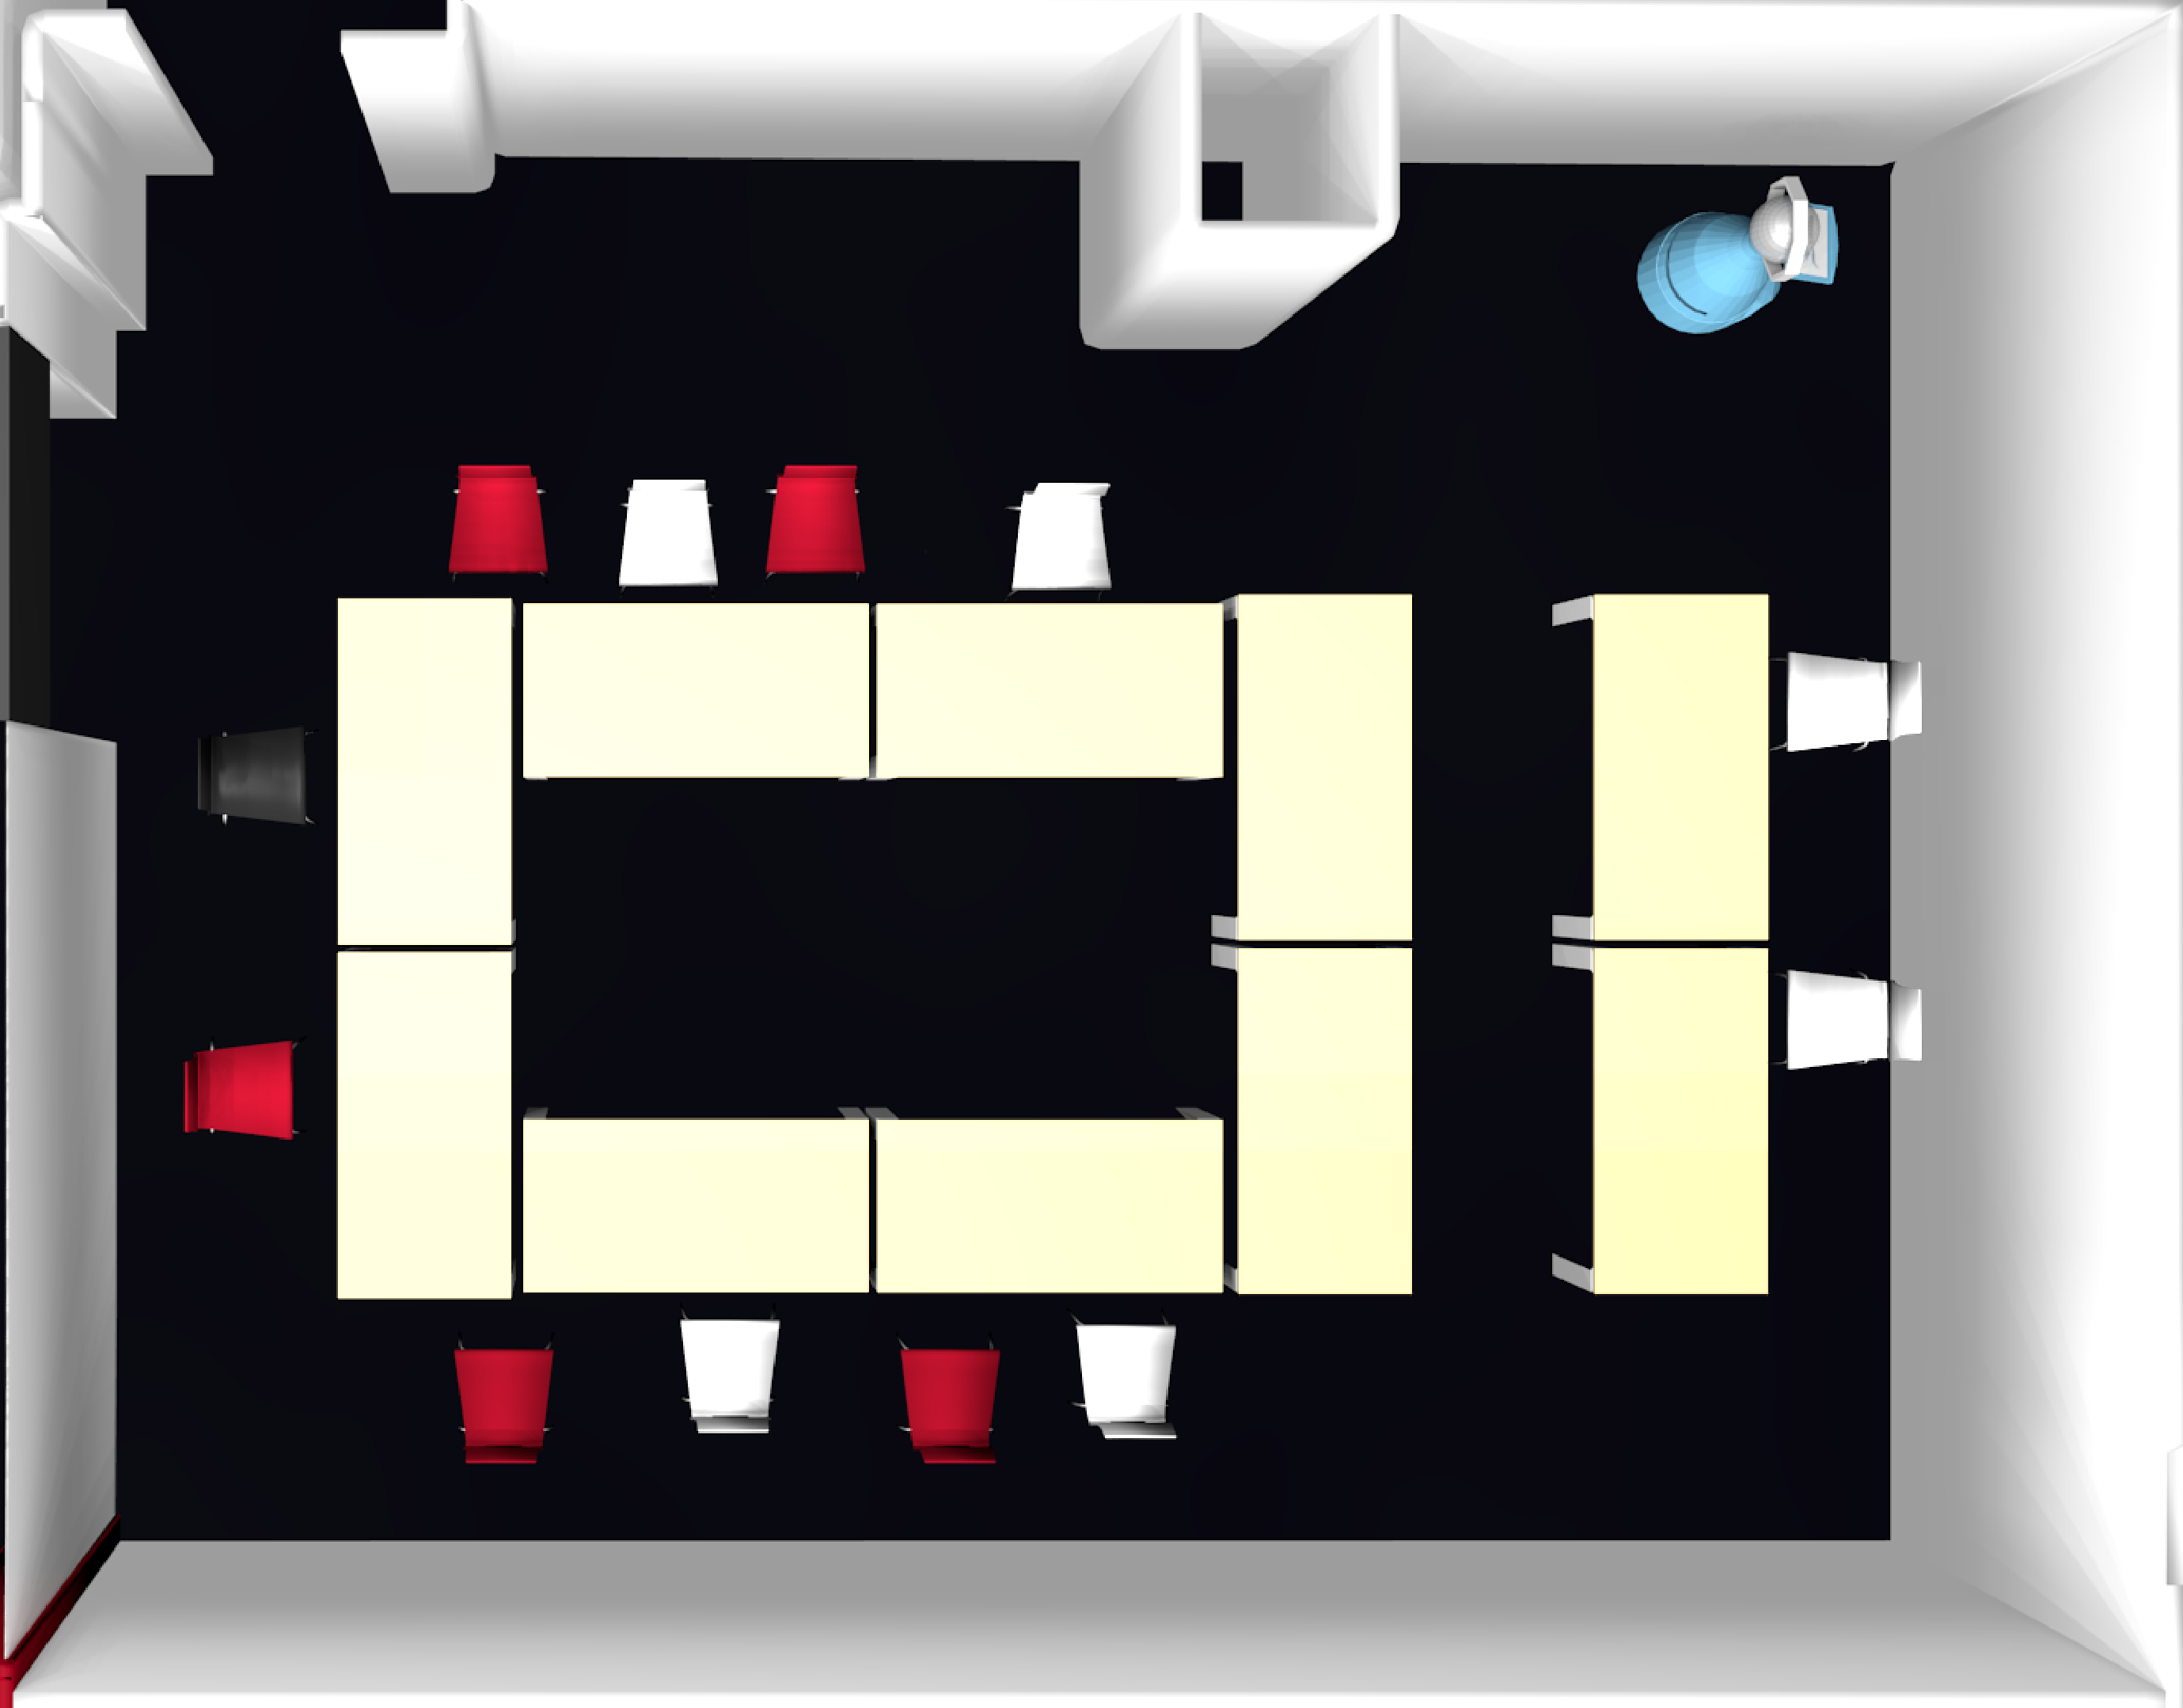
\includegraphics[width=\linewidth]{uol_bl_phase_3_small}
		\caption{One of the rooms in the (simulated) \texttt{uol\_bl} environment. The mobile robot, seen in the top-right, is presented the task of moving from its current location to a location in the main hall, outside the room.}
		\label{fig:uol_bl_tuning_1}
	\end{subfigure}
	\hfill
	\begin{subfigure}{0.475\textwidth}
		\centering
		\vspace{19.5pt}
		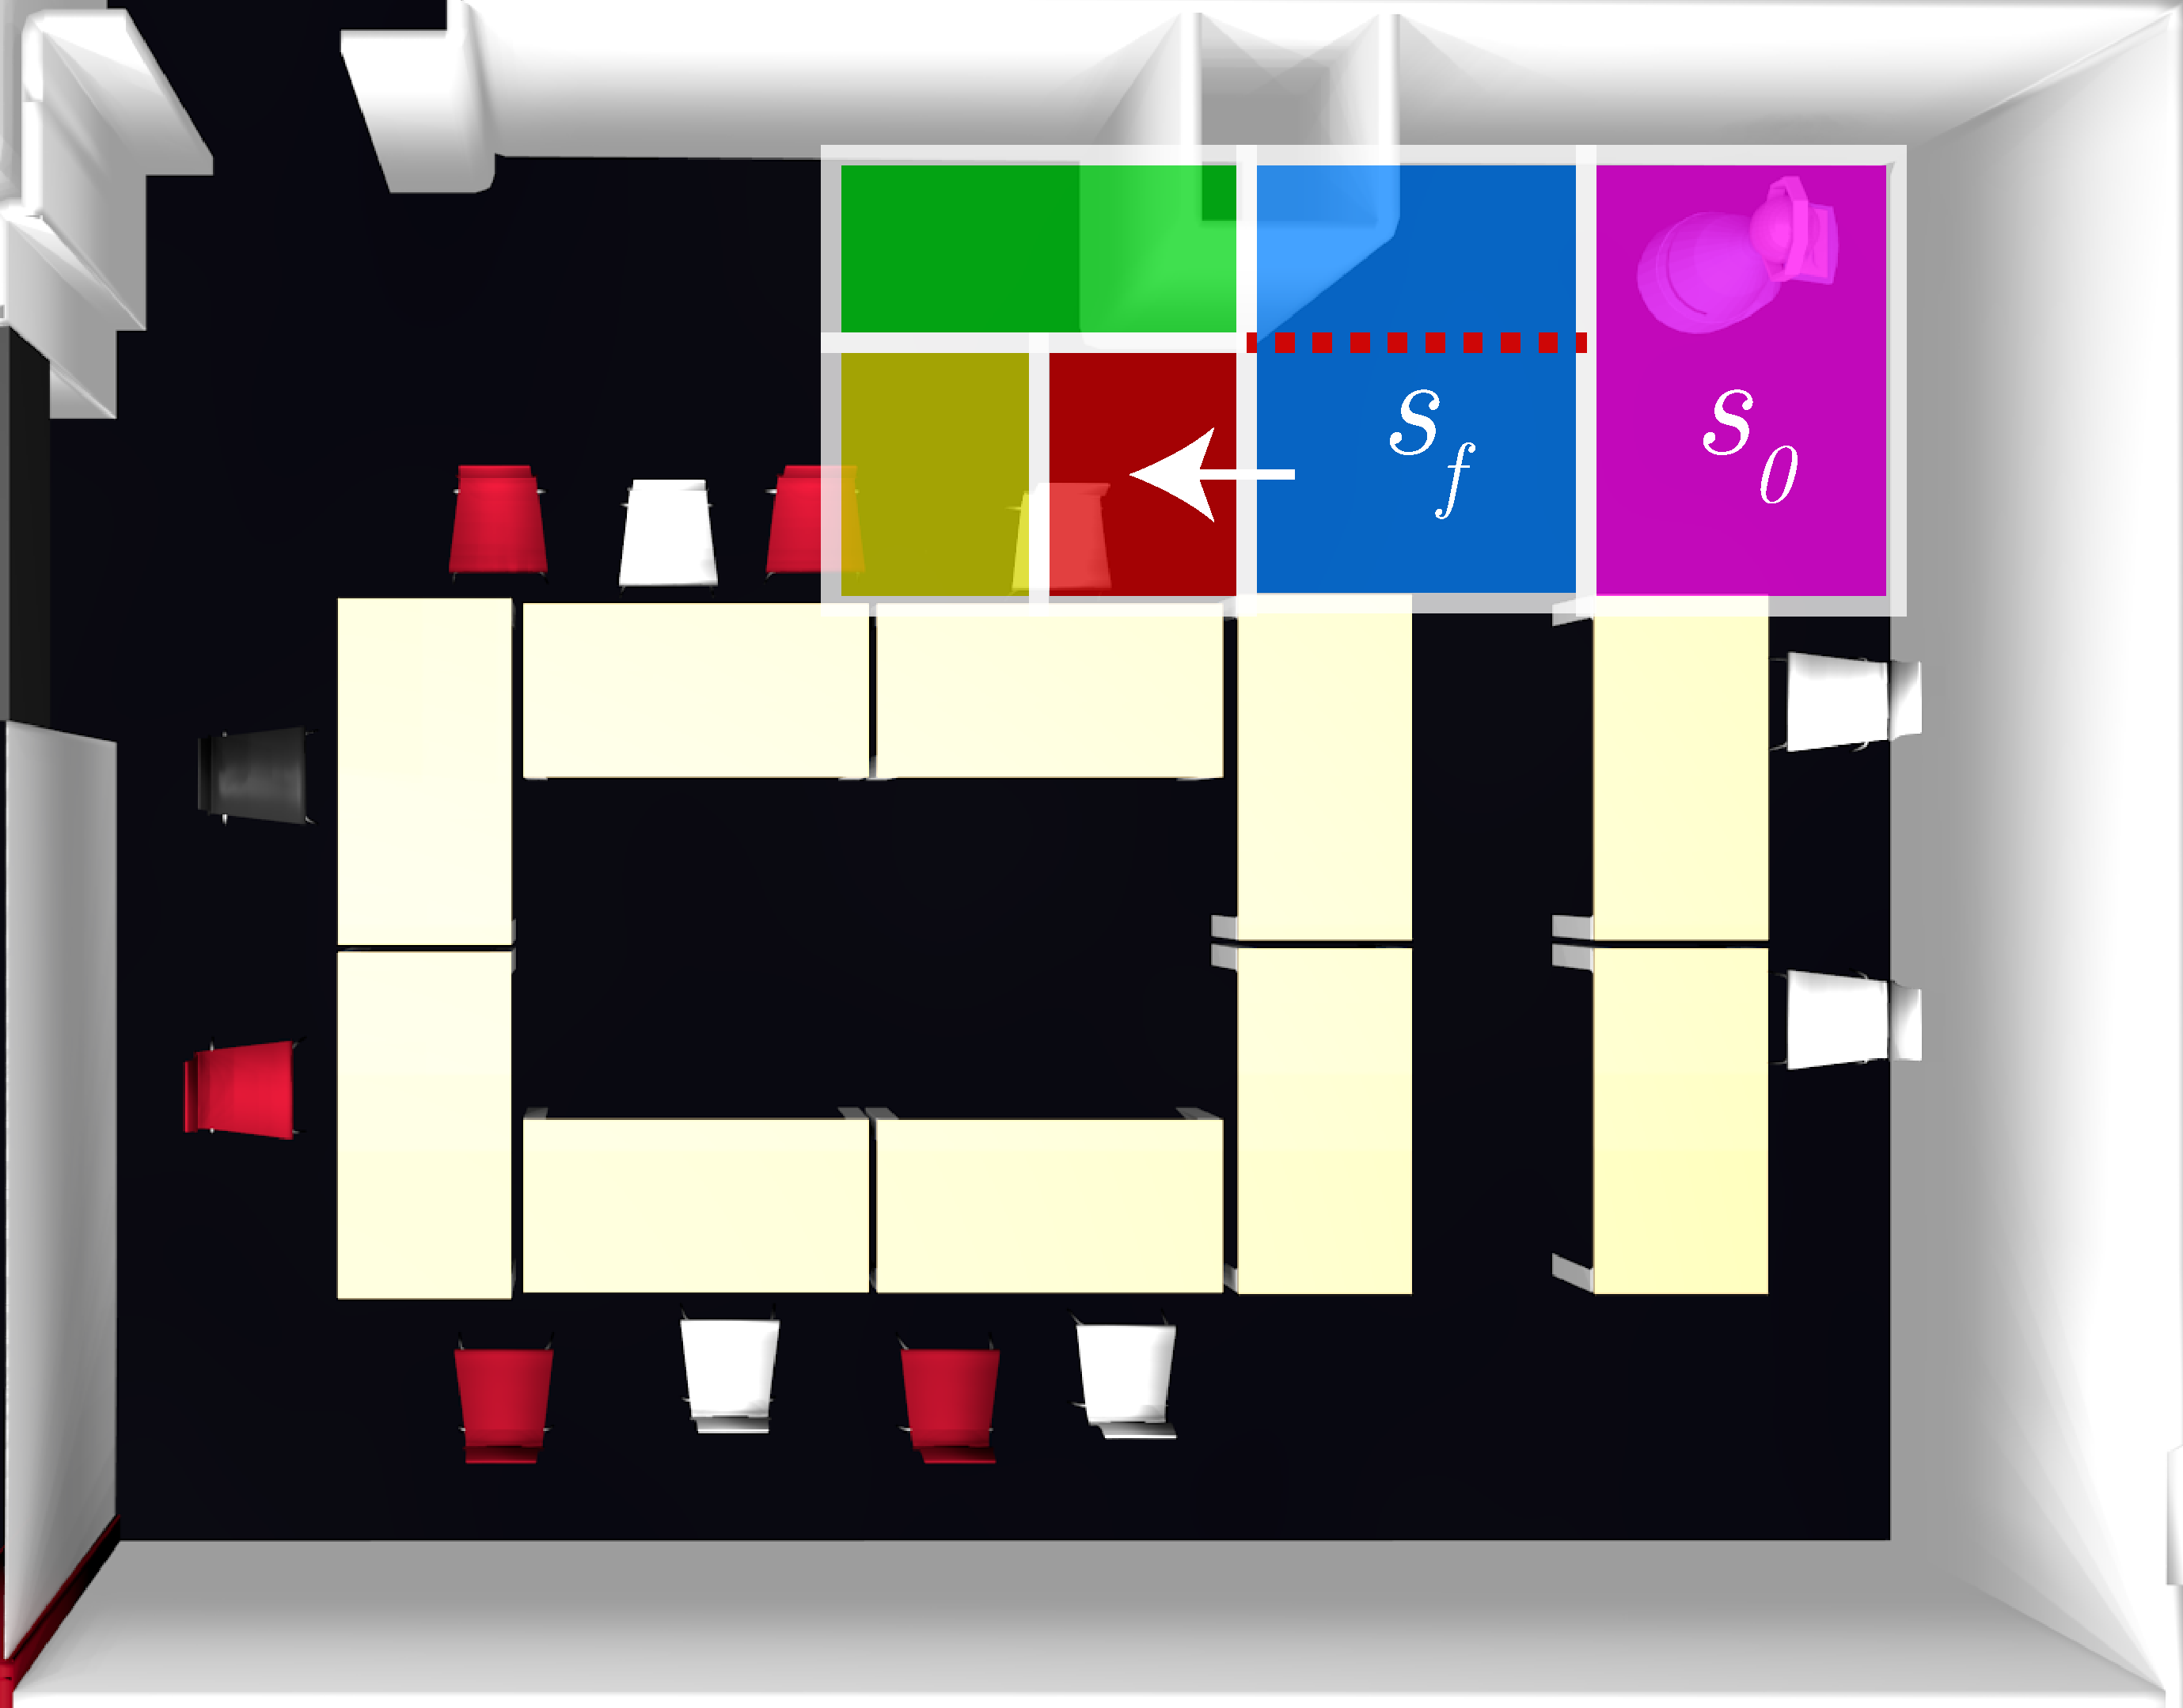
\includegraphics[width=\linewidth]{uol_bl_phase_3_2_smallv6}
		\caption{Illustration of the area of the earlier-learned state space of interest. The resolution for the part of the state space as shown is too low, particularly, considering the state $s_f$, which might cause the robot to get stuck. The third phase of the multi-phase framework therefore splits the state, as depicted by the dotted red line, based on new centroids.}
		\label{fig:uol_bl_tuning_2}
	\end{subfigure}
	\bigskip
	
	\caption{Illustration of the third phase of the multi-phase framework in a simulation of the \texttt{uol\_bl} environment. The phase starts off with the \acrshort{acr:mdp} model learned in the previous phase, and further fine-tunes this model after the robot gets stuck executing a new task.}
	\label{fig:uol_bl_tuning}
\end{figure}

Finally, we get back at the third phase of our multi-phase framework, in which the \acrshort{acr:mdp} $\mathcal{M}$ obtained in the previous phase is further fine-tuned, given a set of new tasks.
To investigate the expediency of this third phase, an implementation of the solution proposed in \autoref{alg:multi-phase-fine-tuning} has been made for the mobile robot navigation application.

Given a task to execute, the solution solves \acrshort{acr:mdp} $\mathcal{M}$ (with new initial state and reward function for this task) for a policy, which it uses to perform the task.
Then, if the controlled robot gets stuck in a state $s_f$ in its attempt to complete the task, it starts to gather new experience about the transitions possible from this state in a collection $E_\mathit{SIM}$.
Based on this new experience, the solution splits the state into a number of new (sub-)states through a clustering of the observations in $E_\mathit{SIM}$, and accordingly updates the transition probabilities based on the new data.
The updated \acrshort{acr:mdp} is then used to compute a new policy for the task, after which the agent tries to perform the task again.
If the agent gets stuck in the same state $s_f$ a clustering with higher resolution is applied to split the state.

For our implementation of this proof-of-concept solution, the mobile robot executes and gathers new experience in a simulation environment.
In gathering new experience, the mobile robot stores the observations (i.e., odometric readings) it makes and the state $s'$ it ends up in after executing an action $a$ from these observations.

To evaluate the approach, we take the \acrshort{acr:mdp} $\mathcal{M}$ learned in the second phase of our last experiment (i.e., see \autoref{fig:exp16}) for the \texttt{uol\_bl} environment.
Then, a new task is presented, which requires the robot to move from the corner of a room in the environment, as shown in \autoref{fig:uol_bl_tuning_1}, to a location in the main hall outside the room.
The problem, is that the resolution in the learned state space $\mathcal{S}$ of $\mathcal{M}$ for this area is too low, as shown in \autoref{fig:uol_bl_tuning_2}, caused by the limited execution traces gathered for this area in the set $E$ used for learning the model.
As a result, there is a considerable chance the robot gets stuck in the state labeled~$s_f \in \mathcal{S}$ from its starting location.

To take care of this, after the observation is made that he robot got stuck, the algorithm makes the robot gather new data about the transitions possible from the different locations within the state $s_f$ in which it got stuck.
Based on this data, the algorithm clusters the data to effectively split the state in two, well-nigh as shown in \autoref{fig:uol_bl_tuning_2}.
The resulting \acrshort{acr:mdp} with updated state space and transition probabilities then allows the mobile robot to successfully accomplish the task (i.e., by the computed policy suggesting to move south and west subsequently).

Although the algorithm works well for fixing small discrepancies like these in the model, caused by limited data about a certain area of the environment, it is not well suited for learning major parts of the model from the ground up.
For such scenarios, one is better off using existing \acrshort{acr:rl} solutions, such as continuous $Q$-learning or active learning approaches which use the learned \acrshort{acr:mdp} as a prior model (see \autoref{sec:active-learning}).